% Options for packages loaded elsewhere
\PassOptionsToPackage{unicode}{hyperref}
\PassOptionsToPackage{hyphens}{url}
\PassOptionsToPackage{dvipsnames,svgnames,x11names}{xcolor}
%
\documentclass[
  10pt,
  dvipsnames,enabledeprecatedfontcommands]{scrartcl}
\usepackage{amsmath,amssymb}
\usepackage{lmodern}
\usepackage{iftex}
\ifPDFTeX
  \usepackage[T1]{fontenc}
  \usepackage[utf8]{inputenc}
  \usepackage{textcomp} % provide euro and other symbols
\else % if luatex or xetex
  \usepackage{unicode-math}
  \defaultfontfeatures{Scale=MatchLowercase}
  \defaultfontfeatures[\rmfamily]{Ligatures=TeX,Scale=1}
\fi
% Use upquote if available, for straight quotes in verbatim environments
\IfFileExists{upquote.sty}{\usepackage{upquote}}{}
\IfFileExists{microtype.sty}{% use microtype if available
  \usepackage[]{microtype}
  \UseMicrotypeSet[protrusion]{basicmath} % disable protrusion for tt fonts
}{}
\makeatletter
\@ifundefined{KOMAClassName}{% if non-KOMA class
  \IfFileExists{parskip.sty}{%
    \usepackage{parskip}
  }{% else
    \setlength{\parindent}{0pt}
    \setlength{\parskip}{6pt plus 2pt minus 1pt}}
}{% if KOMA class
  \KOMAoptions{parskip=half}}
\makeatother
\usepackage{xcolor}
\usepackage{graphicx}
\makeatletter
\def\maxwidth{\ifdim\Gin@nat@width>\linewidth\linewidth\else\Gin@nat@width\fi}
\def\maxheight{\ifdim\Gin@nat@height>\textheight\textheight\else\Gin@nat@height\fi}
\makeatother
% Scale images if necessary, so that they will not overflow the page
% margins by default, and it is still possible to overwrite the defaults
% using explicit options in \includegraphics[width, height, ...]{}
\setkeys{Gin}{width=\maxwidth,height=\maxheight,keepaspectratio}
% Set default figure placement to htbp
\makeatletter
\def\fps@figure{htbp}
\makeatother
\setlength{\emergencystretch}{3em} % prevent overfull lines
\providecommand{\tightlist}{%
  \setlength{\itemsep}{0pt}\setlength{\parskip}{0pt}}
\setcounter{secnumdepth}{5}
\newlength{\cslhangindent}
\setlength{\cslhangindent}{1.5em}
\newlength{\csllabelwidth}
\setlength{\csllabelwidth}{3em}
\newlength{\cslentryspacingunit} % times entry-spacing
\setlength{\cslentryspacingunit}{\parskip}
\newenvironment{CSLReferences}[2] % #1 hanging-ident, #2 entry spacing
 {% don't indent paragraphs
  \setlength{\parindent}{0pt}
  % turn on hanging indent if param 1 is 1
  \ifodd #1
  \let\oldpar\par
  \def\par{\hangindent=\cslhangindent\oldpar}
  \fi
  % set entry spacing
  \setlength{\parskip}{#2\cslentryspacingunit}
 }%
 {}
\usepackage{calc}
\newcommand{\CSLBlock}[1]{#1\hfill\break}
\newcommand{\CSLLeftMargin}[1]{\parbox[t]{\csllabelwidth}{#1}}
\newcommand{\CSLRightInline}[1]{\parbox[t]{\linewidth - \csllabelwidth}{#1}\break}
\newcommand{\CSLIndent}[1]{\hspace{\cslhangindent}#1}
%\documentclass{article}

% %packages
\usepackage{booktabs}
%\usepackage[left]{showlabels}
\usepackage{multirow}
\usepackage{subcaption}

\usepackage{graphicx}
%\usepackage{longtable}
\usepackage{supertabular, booktabs}
\usepackage{ragged2e}
\usepackage{etex}
%\usepackage{yfonts}
\usepackage{marvosym}
\usepackage[notextcomp]{kpfonts}
\usepackage{nicefrac}
\newcommand*{\QED}{\hfill \footnotesize {\sc Q.e.d.}}
\usepackage{floatrow}

\usepackage[textsize=footnotesize]{todonotes}
\newcommand{\ali}[1]{\todo[color=gray!40]{\textbf{Alicja:} #1}}
\newcommand{\mar}[1]{\todo[color=blue!40]{#1}}
\newcommand{\raf}[1]{\todo[color=olive!40]{#1}}

%\linespread{1.5}
\newcommand{\indep}{\!\perp \!\!\! \perp\!}


\setlength{\parindent}{5mm}
\setlength{\parskip}{1pt}


%language
%\usepackage{times}
\usepackage{mathptmx}
\usepackage[scaled=0.86]{helvet}
\usepackage{t1enc}
%\usepackage[utf8x]{inputenc}
%\usepackage[polish]{babel}
%\usepackage{polski}




%AMS
\usepackage{amsfonts}
\usepackage{amssymb}
\usepackage{amsthm}
\usepackage{amsmath}
\usepackage{mathtools}

\usepackage{geometry}
 \geometry{a4paper,left=35mm,top=20mm,}


%environments
\newtheorem{fact}{Fact}



%abbreviations
\newcommand{\ra}{\rangle}
\newcommand{\la}{\langle}
\newcommand{\n}{\neg}
\newcommand{\et}{\wedge}
\newcommand{\jt}{\rightarrow}
\newcommand{\ko}[1]{\forall  #1\,}
\newcommand{\ro}{\leftrightarrow}
\newcommand{\exi}[1]{\exists\, {_{#1}}}
\newcommand{\pr}[1]{\ensuremath{\mathsf{P}(#1)}}
\newcommand{\cost}{\mathsf{cost}}
\newcommand{\benefit}{\mathsf{benefit}}
\newcommand{\ut}{\mathsf{ut}}

\newcommand{\odds}{\mathsf{Odds}}
\newcommand{\ind}{\mathsf{Ind}}
\newcommand{\nf}[2]{\nicefrac{#1\,}{#2}}
\newcommand{\R}[1]{\texttt{#1}}
\newcommand{\prr}[1]{\mbox{$\mathtt{P}_{prior}(#1)$}}
\newcommand{\prp}[1]{\mbox{$\mathtt{P}_{posterior}(#1)$}}



\newtheorem{q}{\color{blue}Question}
\newtheorem{lemma}{Lemma}
\newtheorem{theorem}{Theorem}
\newtheorem{corollary}{Corollary}[fact]


%technical intermezzo
%---------------------

\newcommand{\intermezzoa}{
	\begin{minipage}[c]{13cm}
	\begin{center}\rule{10cm}{0.4pt}



	\tiny{\sc Optional Content Starts}
	
	\vspace{-1mm}
	
	\rule{10cm}{0.4pt}\end{center}
	\end{minipage}\nopagebreak 
	}


\newcommand{\intermezzob}{\nopagebreak 
	\begin{minipage}[c]{13cm}
	\begin{center}\rule{10cm}{0.4pt}

	\tiny{\sc Optional Content Ends}
	
	\vspace{-1mm}
	
	\rule{10cm}{0.4pt}\end{center}
	\end{minipage}
	}
	
	
%--------------------






















\newtheorem*{reply*}{Reply}
\usepackage{enumitem}
\newcommand{\question}[1]{\begin{enumerate}[resume,leftmargin=0cm,labelsep=0cm,align=left]
\item #1
\end{enumerate}}

\usepackage{float}

\usepackage{sectsty}
\sectionfont{\fontsize{11}{11}\selectfont}

% \setbeamertemplate{blocks}[rounded][shadow=true]
% \setbeamertemplate{itemize items}[ball]
% \AtBeginPart{}
% \AtBeginSection{}
% \AtBeginSubsection{}
% \AtBeginSubsubsection{}
% \setlength{\emergencystretch}{0em}
% \setlength{\parskip}{0pt}






\usepackage[authoryear]{natbib}

%\bibliographystyle{apalike}



\usepackage{tikz}
\usetikzlibrary{positioning,shapes,arrows}

\usepackage{booktabs}
\usepackage{longtable}
\usepackage{array}
\usepackage{multirow}
\usepackage{wrapfig}
\usepackage{float}
\usepackage{colortbl}
\usepackage{pdflscape}
\usepackage{tabu}
\usepackage{threeparttable}
\usepackage{threeparttablex}
\usepackage[normalem]{ulem}
\usepackage{makecell}
\usepackage{xcolor}
\ifLuaTeX
  \usepackage{selnolig}  % disable illegal ligatures
\fi
\IfFileExists{bookmark.sty}{\usepackage{bookmark}}{\usepackage{hyperref}}
\IfFileExists{xurl.sty}{\usepackage{xurl}}{} % add URL line breaks if available
\urlstyle{same} % disable monospaced font for URLs
\hypersetup{
  pdftitle={Taking uncertainty in word embedding bias estimation seriously: a bayesian approach},
  pdfauthor={Alicja Dobrzeniecka and Rafal Urbaniak},
  colorlinks=true,
  linkcolor={Maroon},
  filecolor={Maroon},
  citecolor={Blue},
  urlcolor={blue},
  pdfcreator={LaTeX via pandoc}}

\title{Taking uncertainty in word embedding bias estimation seriously: a
bayesian approach}
\author{Alicja Dobrzeniecka and Rafal Urbaniak}
\date{}

\begin{document}
\maketitle

\hypertarget{introduction}{%
\section{Introduction}\label{introduction}}

Natural language processing (NLP) models are used to perform various
language-related tasks such as providing email filters, intelligent
assistants, search results, translations, text analysis and so on. Such
tools require input words to be represented by numbers. This can be done
with word embeddings, which represent words as vectors of real numbers.
A common way to construct an embedding is to use a large natural
language corpus to train a neural network to assign vectors to words
that optimize for co-occurrence prediction accuracy. The vectors can
then be compared in terms of their similarity -- the usual measure is
cosine similarity -- and the results of such comparisons can be used in
downstream tasks. Roughly speaking, cosine similarity is an imperfect
mathematical proxy for semantic similarity {[}14{]}.

It has been suggested {[}1,4,5,8,11,12{]} that such models can learn
implicit biases that reflect harmful stereotypical thinking---for
example, the (vector corresponding to the) word \textit{she} might be
much closer in the vector space to the word \textit{cooking} than the
word \textit{he}. Such phenomena may be undesirable at least in some
downstream tasks, such as web search, recommendations, and so on. To
investigate such issues, several measures of bias in word embeddings
have been formulated and applied. Our goal is to use two prominent
examples of such measures to argue that this approach oversimplifies the
situation and to develop a Bayesian alternative.

One response to the raising of the issue of bias in natural language
models might be to say that there is not much point to reflecting on
such biases, as they are unavoidable. This unavoidability might seem in
line with the arguments to the effect that learning algorithms are
always value-laden {[}9{]}: they employ inductive methods that require
design-, data-, or risk-related decisions that have to be guided by
extra-algorithmic considerations. Such choices necessarily involve value
judgments and have to do, for instance, with what simplifications or
risks one finds acceptable. Admittedly, algorithmic decision making
cannot fulfill the value-free ideal, but this only means that even more
attention needs to be paid to the values underlying different techniques
and decisions, and to the values being pursued in a particular use of an
algorithm.

Another response might be to insist that there is no bias introduced by
the use of machine learning methods here, since the algorithm is simply
learning to correctly predict co-occurrences based on what ``reality''
looks like. However, this objection overlooks the fact that we, humans,
are the ones who construct this linguistic reality, is shaped in part by
the natural language processing tools we use on a massive scale. Sure,
if there is unfairness and our goal is to diagnose it, we should do
complete justice to learning it in the model used in a study thereof.
One example of this approach is {[}3{]}. However, if our goal is to
develop downstream tools that perform tasks that we care about well
without further perpetuating or exacerbating harmful stereotypes, we
still have good reasons to try to minimize the negative impact, at least
as long as this does not damage the overall performance of the tool.
Moreover, it is often not the case that the corpora mirror reality---to
give a trivial example, heads are spoken of more often than kidneys, but
this does not mean that kidneys occur much less often in reality than
heads. To give a more relevant example, the disproportionate association
of female words with female occupations in a corpus actually greatly
exaggerates the actual lower disproportion in the real distribution of
occupations. {[}6{]}.

In what follows, we focus on two popular measures of bias applicable to
many existing word embeddings (
\emph{GoogleNews},\footnote{GoogleNews-vectors-negative300, available at  \url{https://github.com/mmihaltz/word2vec-GoogleNews-vectors}.}
\emph{Glove}\footnote{Available at \url{https://nlp.stanford.edu/projects/glove/}.}
and
\emph{Reddit Corpus}\footnote{The Reddit-L2 corpus, available at  \url{http://cl.haifa.ac.il/projects/L2/}.}):
\emph{Word Embedding Association Test} (WEAT) {[}8{]}, and
\emph{Mean Average Cosine Distance} (MAC) {[}12{]}. We first explain how
these measures are supposed to work. Then we argue that they are
problematic for various reasons, a key one being that by pre-averaging
data they manufacture false confidence, which we illustrate in terms of
simulations showing that the measures often suggest the existence of
bias even if by design it is non-existent in a simulated dataset.

We propose to replace them with a Bayesian data analysis (hierarchical
models), which not only provides more modest and realistic assessment of
the uncertainty involved, but also allows for inspection at various
levels of granularity. Once we introduce the method, we apply it to
multiple word embeddings and results of supposed debiasing, putting
forward some general observations that are not exactly in line with the
usual picture painted in terms of WEAT or MAC (and the problem
generalizes to any approach that focuses on chasing a single numeric
metric): the word list sizes and sample sizes used in the studies are
usually
small,\footnote{Depending on a list for [@Caliskan2017semanticsBiases] the range for protected words is between 13 and 100, and for attributes between 16 and 25; for [@Manzini2019blackToCriminal] the range for protected words is between 14 and 18, and for attributes between 11 and 25}
posterior density intervals are fairly wide, often the differences
between associated, different and neutral human predicates, are not very
impressive. Also, a preliminary inspection suggests that the
desirability of changes obtained by the usual debiasing methods is
debatable. The tools that we have proposed, however, allow for a more
fine-grained and multi-level evaluation of bias and debiasing in
language models without abandoning modesty about the uncertainties
involved.

\hypertarget{two-measures-of-bias-weat-and-mac}{%
\section{Two measures of bias: WEAT and
MAC}\label{two-measures-of-bias-weat-and-mac}}

Conceptually the idea is that if a particular harmful stereotype is
learned in a particular embedding, then certain groups of words will be
systematically closer to (or further from) each other. This gives rise
to the idea of protected groups---for example, in guiding online search
completion or recommendation, female words might require protection in
that they should not be systematically closer to stereotypically female
job names, and male words require protection in that they should not be
systematically closer to toxic masculinity stereotypes, such as
``tough'', ``never complaining'' or ``macho''.\footnote{However, for
  some research-related purposes, such as the study of stereotypes
  across history {[}3{]}, embeddings which do not protect certain
  classes may also be useful.}

The key role in the measures to be discussed is played by the notion of
cosine distance (or, symmetrically, by cosine similarity). These are
defined as follows:\footnote{Here, ``\(-\)'' stands for point-wise
  difference, ``\(\cdot\)'' stands for the dot product operation, and
  \(\lVert a\rVert = \sqrt{(a \cdot a)}\).} \begin{align} \tag{Sim}
\mathsf{cosineSimilarity}(A,B) & = \frac{A \cdot B}{\lVert  A \rVert \,\lVert B \rVert}
\\
\tag{Distance}
\mathsf{cosineDistance}(A,B) &  = 1 - \mathsf{cosineSimilarity}(A,B).
\end{align} Note that this terminology is slightly misleading, as
mathematically cosine distance is not a distance measure, because it
does not satisfy the triangle inequality, as generally
\(\mathsf{cosineDistance}(A,C) \not \leq \mathsf{cosineDistance}(A,B)+ \mathsf{cosineDistance}(B,C)\).
We will keep using this mainstream terminology.

One of the first measures of bias has been developed in {[}1{]}. The
general idea is that a certain topic is associated with a vector of real
numbers (the topic ``direction''), and the bias of a word is
investigated by considering the projection of its corresponding vector
on this direction. For instance, in {[}1{]}, the gender direction
\(\mathsf{gd}\) is obtained by taking the differences of the vectors
corresponding to ten different gendered pairs (such as
\(\overrightarrow{she} - \overrightarrow{he}\) or
\(\overrightarrow{girl} - \overrightarrow{boy}\)), and then identifying
their principal component.\footnote{Roughly, the principal component is
  the vector obtained by projecting the data points on their linear
  combination in a way that maximizes the variance of the projections.}
The gender bias of a word \(w\) is then understood as \(w\)'s projection
on the gender direction: \(\vec{w} \cdot gd\) (which, after normalizing
by dividing by \(\lVert w \rVert \,\lVert \mathsf{gd} \rVert\), is the
same as cosine similarity). Given a list \(N\) of supposedly gender
neutral words,\footnote{We follow the methodology used in the debate in
  assuming that there is a class of words identified as more or less
  neutral, such as \emph{ballpark, eat, walk, sleep, table}, whose
  average similarity to the gender direction (or other protected words)
  is around 0. We will have more to say about this assumption when we
  describe our dataset construction.} and the gender direction
\(\mathsf{gd}\), the direct gender bias is defined as the average cosine
similarity of the words in \(N\) from \(\mathsf{gd}\) (\(c\) is a
parameter determining how strict we want to be): \begin{align*}
\mathsf{directBias_c(N,gd)} & = \frac{\sum_{w\in N}\vert \mathsf{cos}(\vec{w},\mathsf{gd})\vert^c}{\vert N \vert }
\end{align*} \normalsize 

The use of projections in bias estimation has been criticized for
instance in {[}5{]}, where it is pointed out that while a higher average
similarity to the gender direction might be an indicator of bias with
respect to a given class of words, but it is only one possible
manifestation of it, and reducing the cosine similarity to such a
projection may not be sufficient to eliminate bias. For instance,
``math'' and ``delicate'' might be equally similar to a pair of opposed
explicitly gendered words (\emph{she}, \emph{he}), while being closer to
quite different stereotypical attribute words (such as \emph{scientific}
or \emph{caring}). Further, it is observed in {[}5{]} that most word
pairs retain similarity under debiasing meant to minimize
projection-based bias.\footnote{In {[}1{]} another method which involves
  analogies and their evaluations by human users on Mechanical Turk is
  also used. We do not discuss this method in this paper, see its
  criticism in {[}16{]}.}

A measure of bias in word embeddings which does not employ similarities
to pre-calculated protected-class-level directions, the Word Embedding
Association Test (WEAT), has been proposed in {[}8{]}. The idea here is
that the bias between two sets of target words, \(X\) and \(Y\) (we call
them protected words), should be quantified in terms of the cosine
similarity between the protected words and attribute words coming from
two sets of stereotype attribute words, \(A\) and \(B\) (we will call
them attributes). For instance, \(X\) might be a set of male names,
\(Y\) a set of female names, \(A\) might contain stereotypically
male-related, and \(B\) stereotypically female-related career words. The
association difference for a particular word \(t\) (belonging to either
\(X\) or \(Y\)) is:

\vspace{-2mm}

\begin{align*}
\mathsf{s}(t,A,B) & = \frac{\sum_{a\in A}\mathsf{cos}(t,a)}{\vert A\vert} - \frac{\sum_{b\in B}\mathsf{cos}(t,b)}{\vert B\vert}
\end{align*} \normalsize \noindent then, the association difference
between \(A\) a \(B\) is:

\begin{align*}
\mathsf{s}(X,Y,A,B) & = \sum_{x\in X} \mathsf{s}(x,A,B) -  \sum_{y\in Y} \mathsf{s}(y,A,B)
\end{align*}

\noindent The authors use it as a test statistic in some tests, and the
assumption that \(X\) and \(Y\) are of the same size is necessary for
the statistic to make sense. In the final measure (of effect size),
WEAT, means are taken, which makes it insensitive to size differences
between \(X\) and \(Y\): \begin{align}
\mathsf{weat}(A,B) & = \frac{
\mu(\{\mathsf{s}(x,A,B)\}_{x\in X}) -\mu(\{\mathsf{s}(y,A,B)\}_{y\in Y}) 
}{
\sigma(\{\mathsf{s}(w,A,B)\}_{w\in X\cup Y})
}
\end{align}

WEAT is inspired by the Implicit Association Test (IAT) {[}17{]} used in
psychology, and it uses almost the same word sets, allowing for a
\emph{prima facie} sensible comparison with bias in humans. In {[}8{]}
the authors argue that significant biases---thus measured--- similar to
the ones discovered by IAT can be discovered in word embeddings. In
{[}11{]} the methodology is extended to a multilingual and cross-lingual
setting, arguing that using Euclidean distance instead of cosine
similarity does not make much difference, while the bias effects vary
greatly across embedding models (interestingly, with social media-text
trained embeddings being less biased than those based on Wikipedia). A
similar methodology is employed in {[}4{]}. The authors employ word
embeddings trained on corpora from different decades to study the shifts
in various biases.\footnote{Strictly speaking, these authors use
  Euclidean distances and their differences, but the way they take
  averages and averages thereof is analogous, and so what we will have
  to say about pre-averaging leading to false confidence applies to this
  methodology as well.}

WEAT, however, has been developed to investigate biases corresponding to
a pair of supposedly opposing stereotypes, and so the question arises as
to how generalize the measure to contexts in which biases with respect
to more than two stereotypical groups are to be measured. Such a
generalization can be found in {[}12{]}. The authors introduce Mean
Average Cosine distance (MAC) as a measure of bias. Let
\(T = \{t_1, \dots, t_k\}\) be a set of protected words, and let each
\(A_j\in \mathcal{A}\) be a set of attributes stereotypically associated
with a protected word where \(\mathcal{A}\). For instance, when biases
related to religion are to be investigated, they use a dataset of the
format illustrated in Table \ref{tab:religionOriginal}. The measure is
defined as follows:

\begin{table}
\footnotesize

\centering

\begin{tabular}[t]{lllr}
\toprule
protected words ($T$) & attributes & attribute set ($A_j$) & cosine distance\\
\midrule
\cellcolor{gray!15}{rabbi} & \cellcolor{gray!15}{greedy} & \cellcolor{gray!15}{jewStereotype} & \cellcolor{gray!15}{1.0306175}\\
church & familial & christianStereotype & 0.7087424\\
\cellcolor{gray!15}{synagogue} & \cellcolor{gray!15}{liberal} & \cellcolor{gray!15}{jewStereotype} & \cellcolor{gray!15}{0.7922607}\\
jew & familial & christianStereotype & 0.9783245\\
\cellcolor{gray!15}{quran} & \cellcolor{gray!15}{dirty} & \cellcolor{gray!15}{muslimStereotype} & \cellcolor{gray!15}{1.1207093}\\
muslim & uneducated & muslimStereotype & 0.5160429\\
\cellcolor{gray!15}{torah} & \cellcolor{gray!15}{terrorist} & \cellcolor{gray!15}{muslimStereotype} & \cellcolor{gray!15}{0.9341137}\\
quran & hairy & jewStereotype & 1.1764642\\
\cellcolor{gray!15}{synagogue} & \cellcolor{gray!15}{violent} & \cellcolor{gray!15}{muslimStereotype} & \cellcolor{gray!15}{0.9549743}\\
bible & cheap & jewStereotype & 1.2234364\\
\cellcolor{gray!15}{christianity} & \cellcolor{gray!15}{greedy} & \cellcolor{gray!15}{jewStereotype} & \cellcolor{gray!15}{0.9728545}\\
muslim & hairy & jewStereotype & 0.8788219\\
\cellcolor{gray!15}{islam} & \cellcolor{gray!15}{critical} & \cellcolor{gray!15}{christianStereotype} & \cellcolor{gray!15}{0.7880706}\\
muslim & conservative & christianStereotype & 0.4453191\\
\cellcolor{gray!15}{mosque} & \cellcolor{gray!15}{greedy} & \cellcolor{gray!15}{jewStereotype} & \cellcolor{gray!15}{1.1541524}\\
\bottomrule
\end{tabular}

\caption{Sample 15 rows of the religion dataset. The whole dataset has 15 unique protected words ($T$), and 11 unique attributes divided between 3 attribute sets ($A_1=\mathsf{jewStereotype}, A_2= \mathsf{christianStereotype}, A_3=\mathsf{muslimStereotype}$). $\mathcal{A}$ consists of these three sets, $\mathcal{A}= \{A_1, A_2, A_3\}$. The whole dataset has $15\times 11 = 165$ rows.}
\label{tab:religionOriginal}
\normalsize 
\end{table}

\begin{align*}
\mathsf{s}(t, A_j) & = \frac{1}{\vert A_j\vert}\sum_{a\in A_j}\mathsf{cosineDistance}(t,a) \\
\mathsf{mac}(T,\mathcal{A}) & = \frac{1}{\vert T \vert \,\vert \mathcal{A}\vert}\sum_{t \in T }\sum_{A_j \in \mathcal{A}}    \mathsf{s}(t,A_j)
\end{align*}

\noindent That is, for each protected word \(t\in T\), and each
attribute set \(A_j\), they first take the mean of distances for this
protected word and all attributes in a given attribute class, and then
take the mean of thus obtained means for all the protected words and all
the protected classes.\footnote{The authors' code are in their github
  repository,
  \url{https://github.com/TManzini/DebiasMulticlassWordEmbedding}.}

Having introduced the measures, first, we will introduce a selection of
general problems with this approach, and then we will move on to more
specific but important problems related to the fact that the measures
take averages and averages of averages. Once this is done, we move to
the development of our Bayesian alternative and the presentation of its
deployment.

\hypertarget{general-methodological-problems-with-cosine-based-measures-of-bias}{%
\section{General methodological problems with cosine-based measures of
bias}\label{general-methodological-problems-with-cosine-based-measures-of-bias}}

Consider the MAC results from Table REF. Are the initial MAC values
lower than 1 indicative of the presence of bias? Of course, thinking
abstractly, 1 is the ideal distance for unrelated words. But clearly,
there is variation in distances, which might lead to non-biased lists
also having MAC smaller than 1. How much smaller? While the original
paper did not employ control lists for comparison in the paper. To
obtain a more realistic gauge on how to understand MAC values (and in
further development of our approach), we introduced control word lists.
One of them is a list of words we intuitively considered neutral (see
REF in the APPENDIX). Moreover, it might be the case that words that
have to do with human activities are systematically closer to the
protected words than merely neutral words, for which reason we also use
a second list with intuitively non-stereotypical human attributes (see
REF in the APPENDIX). Another important observation is that in their
calculations the authors do not distinguish whether a given attribute is
associated with a given protected word (e.g.~protected word \emph{jew}
and the attribute \emph{greedy}) or whether it is associated with a
different stereotype from the same list (e.g.~protected word
\emph{quran} and the attribute \emph{greedy}), simply averaging across
all such groups.

In Figure \ref{fig:empirical} We look at the empirical distributions,
while paying attention to such divisions. Horizontal lines represent
1-MAC values that the authors considered indicative of bias for
stereotypes corresponding to given word lists. For instance, in
religion, MAC was .859, so we plot \(0\pm (1-.859)\approx .14\) lines
around similarity = 0 (that is, distance = 1). Notice that most
distributions are quite wide, and the proportions of even neutral or
human neutral words with similarities higher than the value of 1-MAC
deserving debiasing according to the authors is quite high.

\pagebreak

\begin{figure}[H]

\begin{center}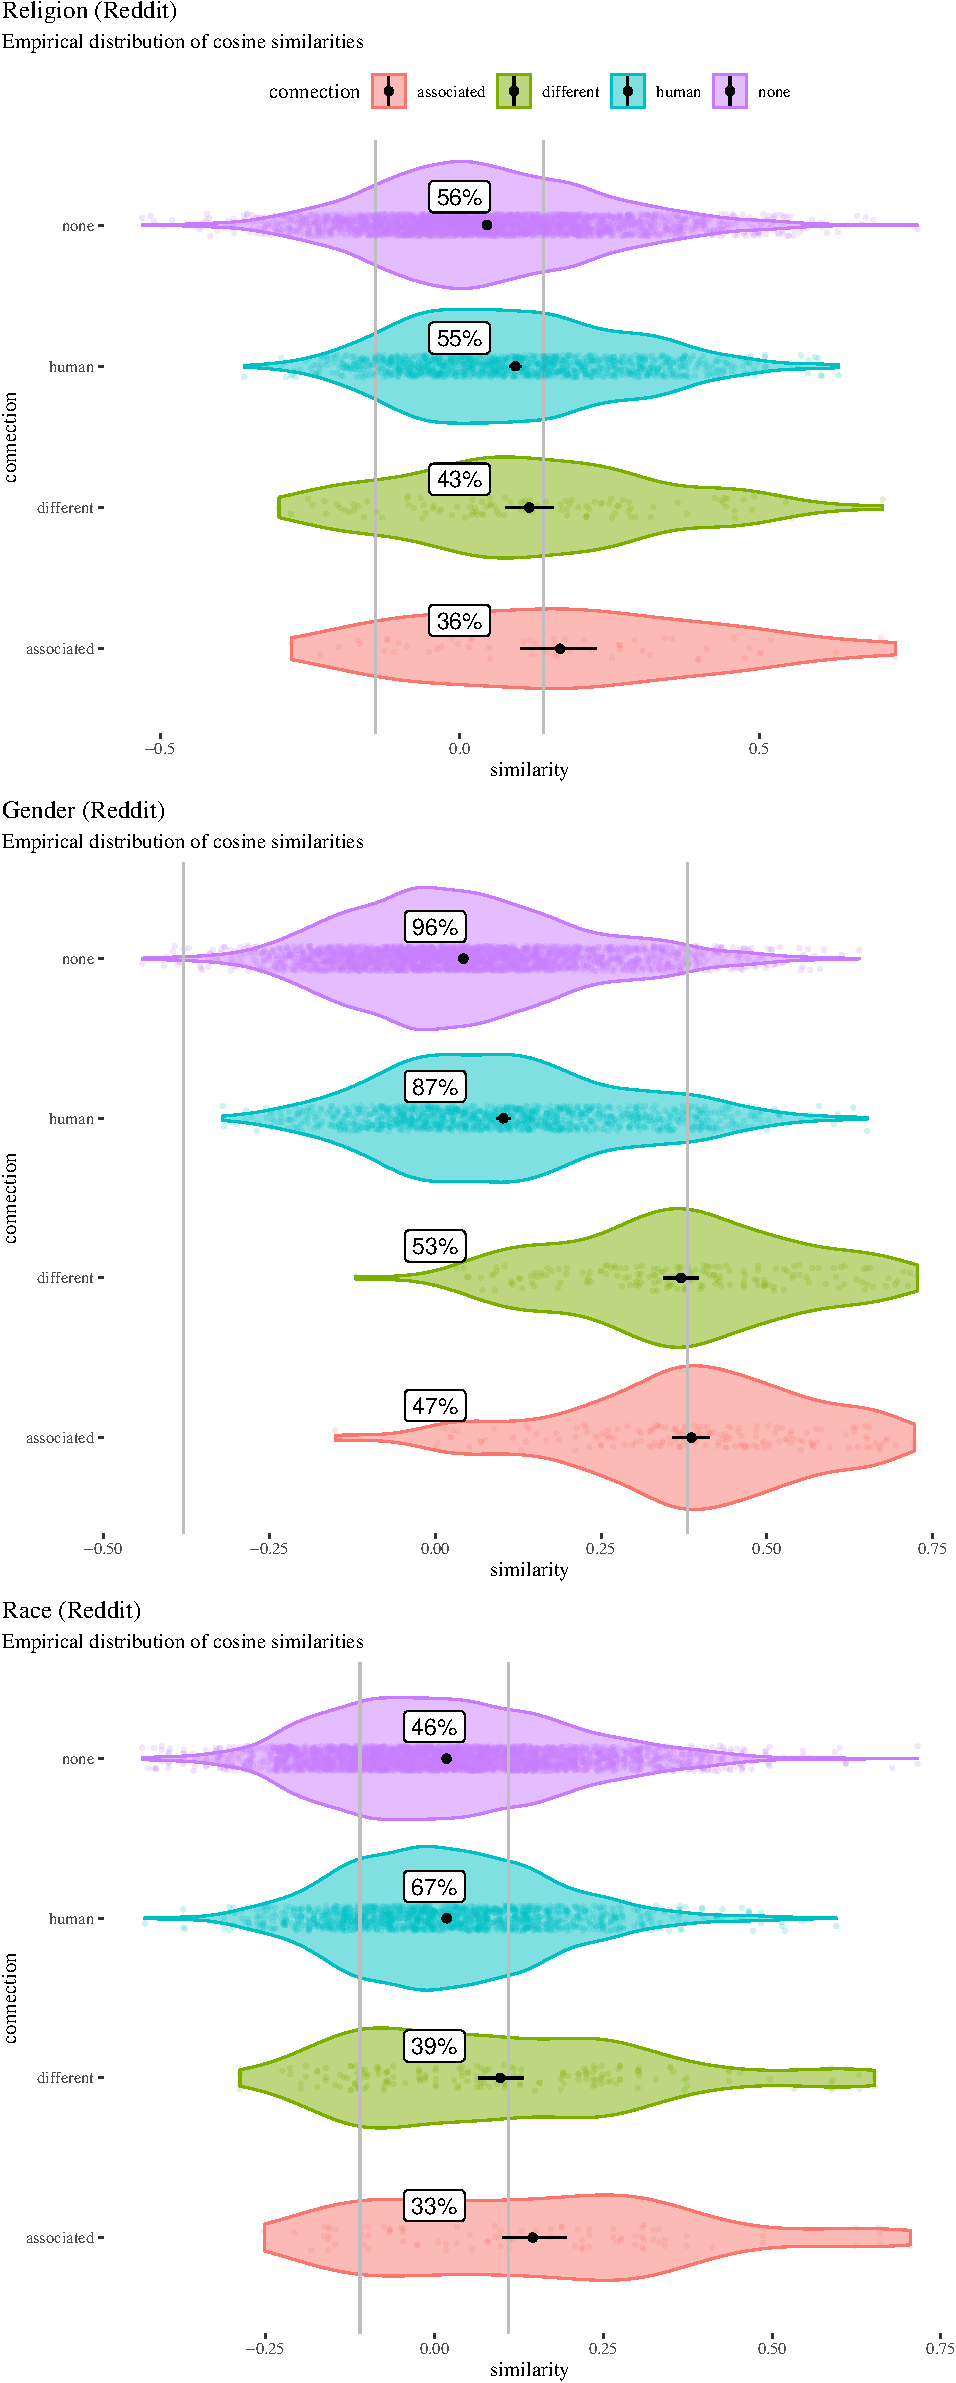
\includegraphics[width=0.7\linewidth]{paperDraft_files/figure-latex/fig:cosineDistributions8b-1} \end{center}

\caption{Empirical distributions of cosine similarities (1-distances) for three word lists used in  the original paper.  }

\label{fig:empirical}
\end{figure}

One issue to consider is the selection of attributes for bias
measurement. The word lists used in the literature are often fairly
small (5-50).

While the papers do employ statistical tests to measure the uncertainty
involved, we will later on argue that these method are not proper for
the goal at hand and show that a more appropriate use of statistical
methods leads to estimates of uncertainty that are rather
epistemologically pessimistic. \todo{sensitivity to choice of words}

Let's think about MAC, using the case of religion-related stereotypes.
The full lists from {[}12{]} can be found in
\ref{appendix:manzini_word_lists}. In the original paper, words from all
three religions were compared against all of the stereotypes. One reason
this is problematic is that no distinction between cases in which the
stereotype is associated with a given religion, as opposed to the
situation in which it is associated with another one, is made. This is
problematic, as not all of the stereotypical words have to be considered
as harmful for all of the religions. One should investigate the
religions separately as some of them may have stronger harmful
associations that others.

The interpretation of the results is also a challenge. In {[}12{]} we
can find summaries of average cosine distances per group (such as
gender, race, or religion). For instance, for religion, here is the
relevant fragment of table:

\begin{table}
\footnotesize

\centering

\begin{tabular}[t]{lllr}
\toprule
Religion Debiasing & MAC & a p-value \\
\midrule
\cellcolor{gray!15}{Biased} & \cellcolor{gray!15}{0.859} & \cellcolor{gray!15}{N/A} \\
Hard Debiased & 0.934 & 3.006e-07\\
\cellcolor{gray!15}{Soft Debiased ($\lambda$ = 0.2)} & \cellcolor{gray!15}{0.894} & \cellcolor{gray!15}{0.007} \\
\bottomrule
\end{tabular}

\caption{The associated mean average cosine similarity
(MAC) and p-values for debiasing methods for religious bias}
\label{tab:religionOriginal2}
\normalsize 
\end{table}

\noindent (MAC stand for mean average cosine similarity, although in
reality the the table contains mean cosine distances). What may attract
attention is the fact that the value of cosine distance in ``Biased''
category is already quite high (i.e.~close to 1) even before debiasing.
High cosine distance indicates low cosine similarity between values. One
could think that average cosine similarity equal to approximately 0.141
is not significant enough to consider it as bias. However, the authors
still aim to mitigate such ``bias'' to make the distance even larger.
Methodologically the question is, on what basis is this small similarity
still considered as a proof of the presence of bias, and whether these
small changes are meaningful.

The underlying problem here is that in the paper there is no control
group. One should also include control groups to have a way of comparing
the results for a supposedly stereotyped group with the results for sets
of neutral or human-related neutral words. In our approach later on, we
distinguish between stereotypes associated with a given group,
stereotypes associated with different groups, and introduce control
groups: neutral words and stereotype-free human predicates.

\hypertarget{metrics-that-pre-average-are-a-bad-guide}{%
\subsection{Metrics that pre-average are a bad
guide}\label{metrics-that-pre-average-are-a-bad-guide}}

In contrast, statistical intervals will help us decide whether a given
cosine similarity is high enough to consider the words to be more
similar than if we chose them at random. We will use highest posterior
density intervals, in line with Bayesian methodology.

Crucially, these approaches use means of mean average cosine
similarities to measure similarity between protected word and harmful
stereotypes. If one takes a closer look at the individual values that
are taken for the calculations, it turns out that there are quite a few
outliers and surprisingly dissimilar words. This problem becomes
transparent when we examine the visualizations of the individual cosine
distances, following the idea that one of the first steps in
understanding data is to look at it.

With such a method the uncertainty involved is not really considered
which makes it even more difficult to give reasonable interpretations of
the results. We propose the use of Bayesian method to obtain some
understanding of the influence the uncertainty has on the interpretation
of final results.

\noindent \(s(X,Y,A,B)\) is the statistic used in the significance test,
and the \(p\)-value is obtained by bootstrapping: it is the frequency of
\(s(X_i,Y_i,A,B)>s(X,Y,A,B)\) for all equally sized partitions
\(X_i, Y_i\) of \(X\cup Y\). The effect size is computed by normalizing
the difference in means as follows:

\vspace{-2mm}

\footnotesize

\begin{align}
bias(A,B) & = \frac{
\mu(\{s(x,A,B)\}_{x\in X}) -\mu(\{s(y,A,B)\}_{y\in Y}) 
}{
\sigma(\{s(w,A,B)\}_{w\in X\cup Y})
}
\end{align}

\normalsize

The t-tests they employ are run on average cosines used to calculate
MAC.

\hypertarget{pre-averaging-bootstrapping-and-testing-with-the-null-model}{%
\section{Pre-averaging, bootstrapping and testing with the null
model}\label{pre-averaging-bootstrapping-and-testing-with-the-null-model}}

The effect sizes reported by {[}8{]} for lists of words for which the
embeddings are supposedly biased range from 2.06 to 1.81, and the
reported \(p\)-values are in the range of \(10^{-7}-10^{-2}\) with one
exception for Math vs arts, where it is \(.018\). The question is, are
those results meaningful?

One way to answer this question is to think in terms of null models. If
the words actually are samples from two populations with equal mean, how
often would we see effect sizes in this range? How often would we reach
the \(p\)-values that the authors reported?

We start our exploration with considering a list of 16 protected words,
each class containing 8, with 16 attributes, 8 in each attribute class.
In each particular sample we will investigate the consequence of the
model being in fact null: we draw the cosine distances, every time, from
the \(\mathsf{Normal}(0,.08)\) distribution. \(0.08\) is approximately
the empirical standard deviation observed in fairly large samples of
neutral words, and 16 is the sample size used in the WEAT7 word list,
which is not much different from the other sample sizes in word lists
used by {[}8{]}

So let's draw one sample of this type. We calculate the s-values, the
test statistics and the effect sizes. Then, following the original
methodology, we obtain bootstrapped distributions of the effect sizes
and the test statistics by calculating the same for each possible equal
split of the initial random data set. The observed test statistic is
0.386222 and 1.2671948. The bootstrapped distributions of the test
statistics and effect sizes are illustrated in Figure
\ref{fig:caliskanCalc}. Quite notably both (two-sided) \(p\) values are
uneven and rather low.

\begin{figure}[H]

\begin{center}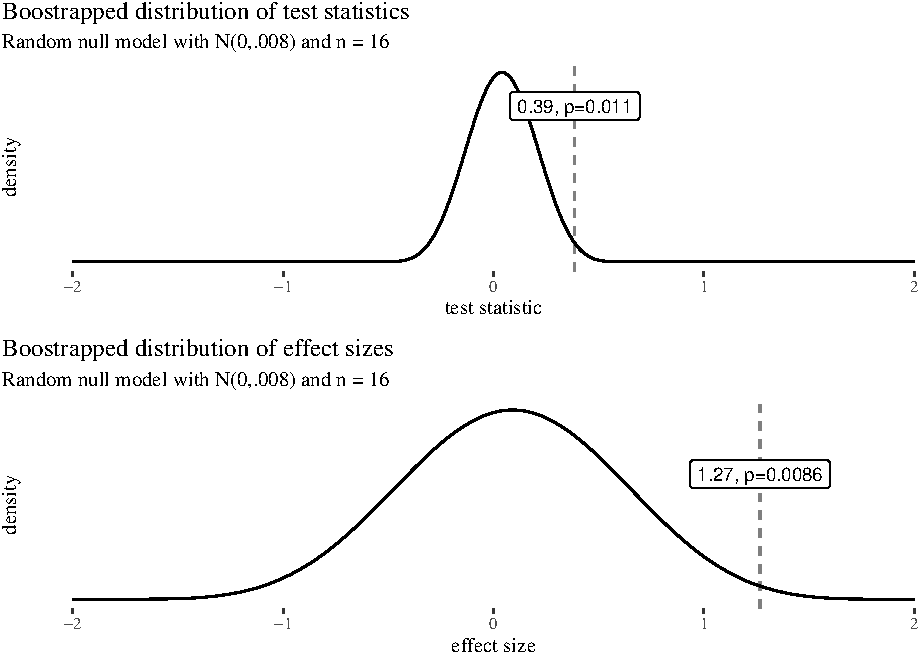
\includegraphics[width=0.8\linewidth]{paperDraft_files/figure-latex/fig:caliskanCalcB2B-1} \end{center}

\caption{Bootstrapped distributions of test statistics and effect sizes in a random sample given the null hypothesis.}
\label{fig:caliskanCalc}
\end{figure}

At this point, we might think---right, so while drawing on the
assumption of the null hypothesis we just stumbled into a data set that
randomly happened to display strong bias. We decide to double-check this
by visual inspection expecting exactly this: a strong, clearly visible
bias (Figure \ref{fig:caliskanDistances}).

\begin{figure}[H]

\begin{center}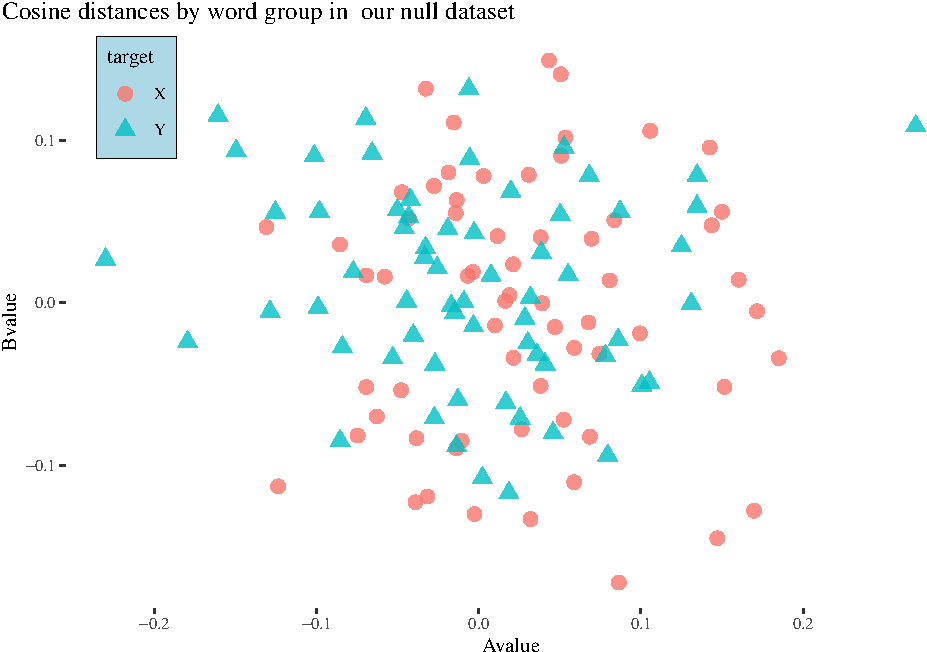
\includegraphics[width=0.8\linewidth]{paperDraft_files/figure-latex/fig:caliskanDistC2B-1} \end{center}

\caption{Cosine distances to two attribute sets by protected word groups. Observe nothing unusual except for a few outliers.}
\label{fig:caliskanDistances}
\end{figure}

\noindent In fact, while there might be some outliers here and there,
saying that a clear bias on which one group is systematically closer to
\(A\)s than another is definitely a stretch. What happened?

In the calculations of WEAT means are taken twice. The \(s\)-values
themselves are means, and then means of \(s\)-values are compared
between groups. The test statistic used itself is of this sort as
well---while it compares sums, these are sums of sets of the same size,
so they are really linear transformations of means of means. Statistical
troubles start when we run statistical tests on sets of means, for at
least two reasons One, by pre-averaging data we throw away information
about sample sizes. For the former point, think about proportions: 10
out of 20 and 2 out of 4 give the same mean, but you would obtain more
information by making the former observation rather than by making the
latter. And especially in this context, in which the word lists are not
huge, sample sizes should matter. Two, when we pre-average, we remove
variation, and so pre-averaging tend to manufacture false confidence.
Group means display less variation than the raw data points, and the
standard deviation of a set of means of sets of means is bound to be
lower than the original standard deviation in the row data. Now, if you
calculate your effect size by dividing by the pre-averaged standard
deviation, your quite likely to get something that looks like a strong
effect size, but the results of your calculations might not track
anything interesting.

So let us think again about the question that we are ultimately
interested in. Are the \(X\) terms systematically closer to (further
from) the \(A\) attributes (\(B\) attributes) than the \(Y\) words? But
now let's use the raw data points to try to answer these questions. As
the first stab, let us run two quick \(t\)-tests to gauge what the raw
data illustrated in Figure \ref{fig:caliskanDistances} tell us.

First, distances to \(A\) attributes for \(X\) words and \(Y\) words.
Whoa, the result is significant! The \(p\)-value is \(0.02\). So sure,
the sample is in some sense unusual. But the 95\% confidence interval
for the difference in means is \([.0052 .061]\), clearly nothing that a
reader would expect given that the calculated effect size seemed quite
large. How about the \(B\) attributes? Here the \(p\)-value is \(.22\)
and the 95\% confidence interval is \([-0.03, .009]\), even less of a
reason to think a bias is present.

The difficulties are exacerbated by the fact that statistical tests are
based on bootstrapping from a relatively small data sets, which is quite
likely to underestimate the population variance. To make our point
clear, let us avoid bootstrapping and work with the null generative
model with \(\mathsf{Norm}(0,.08)\) for both word groups. We keep the
sizes the same: we have eight protected words in each group, sixteen in
total, and for each we randomly draw 8 distances from hypothetical \(A\)
attributes, and \(8\) distances from hypothetical \(B\) attributes.
Calculate the test statistic and effect size the way {[}8{]} did. Do
this 10000 times and look at what the distributions of these values are
on the assumption of the null model with realistic empirically motivated
raw data point standard deviation.

\begin{figure}[H]

\begin{center}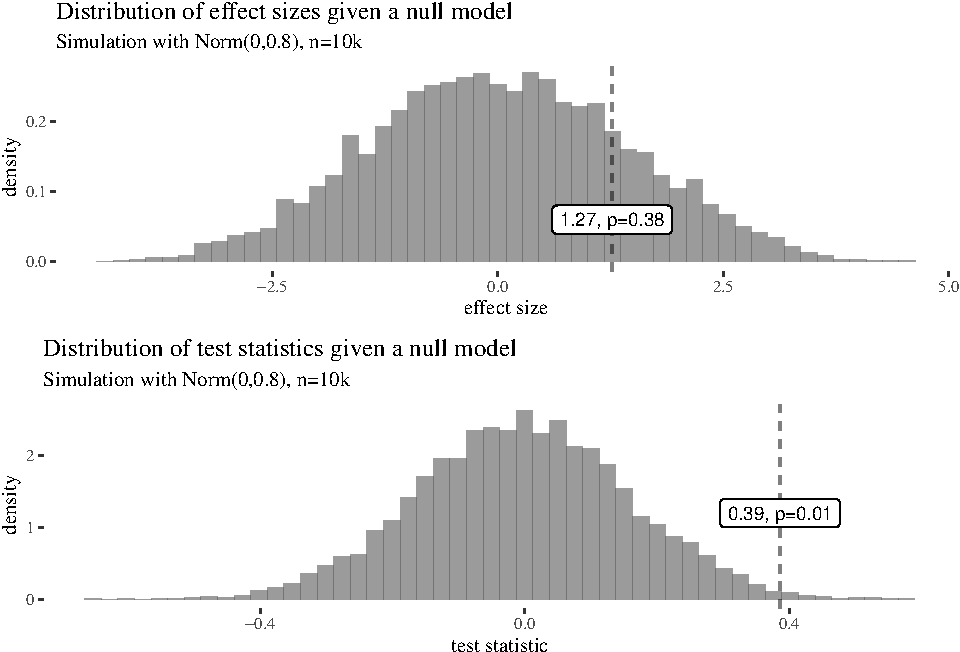
\includegraphics[width=0.8\linewidth]{paperDraft_files/figure-latex/fig:ourDistancesPlot2-1} \end{center}

\caption{Distributions of test statistics and effect sizes based on 10k simulations on the assumption of a null model in which all distances come from normal distribution with $\mu =0, \sigma = .08$.}
\label{fig:ourDistances}
\end{figure}

The first observation is that the supposedly large effect size we
obtained is not that unusual even assuming a null model. Around 38\% of
samples result in effect size at least as extreme. This illustrates the
point that the effect size used does not track anything interesting.
Second, the distribution of test statistics is much more narrow, which
means that if we use it to calculate \(p\)-values, it is not too
difficult to obtain a supposedly significant test statistic which
nevertheless does not correspond to anything interesting happening in
the data set.

Where do we stand now? We have seen that seemingly high effect sizes
might arise even if the underlying processes actually have the same
mean. The uncertainty resulting from including the raw data point
variance into considerations is more extensive than the one suggested by
the low p-values obtained from taking means or means of means as data
points. In this section, we discussed the performance of the WEAT
measure, but since the {[}12{]} one is a generalization thereof,
including the method of running statistical tests on pre-averaged data,
our remarks, \emph{mutatis nutandis}, apply. Moreover, a general problem
is that studies such as {[}8{]} or {[}12{]} do not use control groups,
and this makes the interpretation of the analysis additionally
difficult.

What is the alternative? As we already emphasized: focusing on what the
real underlying question is, and trying to answer it using a statistical
analysis of the raw data. Moreover, since the data sets are not too
large and since multiple evaluations are to be made, we will pursue this
method from the Bayesian perspective.

\hypertarget{bayesian-method}{%
\section{Bayesian method}\label{bayesian-method}}

\hypertarget{introduction-and-model-definition}{%
\subsection{Introduction and model
definition}\label{introduction-and-model-definition}}

Bayesian data analysis takes prior probability distributions, a
mathematical model structure and the data, and returns the posterior
probability distributions over the parameters of interest, thus
capturing our uncertainty about their actual values. One important
difference between such a result and the result of a classical
statistical analysis is that classical confidence intervals (CIs) have a
rather complicated and somewhat confusing interpretation, which has
little to do with the posterior probability distribution.\footnote{Here
  are a few usual problems. CIs are often mistakenly interpreted as
  providing the probability that a resulting confidence interval
  contains the true value of a parameter. CIs bring confusion also with
  regard to precision, it is a common mistake to interpret narrow
  intervals as the ones corresponding to a more precise knowledge.
  Another fallacy is to associate CIs with likelihood and stating that
  values within a given interval are more probable than the ones outside
  it. The theory of confidence intervals does not support the above
  interpretations. CIs should be plainly interpreted as a result of
  certain procedure (there are many ways to obtain CIs from a given set
  of data) that will in the long run contain the true value if the
  procedure is performed a fixed amount of times. For a nice survey and
  explanation of these misinterpretations, see {[}15{]}. For a
  psychological study of the occurrence of such misinterpretations, see
  REF. In this study, 120 researchers and 442 students were asked to
  assess the truth value of six false statements involving different
  interpretations of a CI. Both researchers and students endorsed, on
  average, more than three of these statements.} {[}7{]}

In fact, Bayesian highest posterior density intervals (HPDIs, the
narrowest intervals containing a certain ratio of the area under the
curve) and CIs end up being numerically the same only if the prior
probabilities are uniform. This illustrates that (1) classical analysis
is unable to incorporate non-trivial priors, and (2) is therefore more
susceptible to over-fitting, unless regularization (equivalent to a more
straightforward Bayesian approach) is used. In contrast with CIs, the
posterior distributions are easily interpretable and have direct
relevance for the question at hand. Moreover, Bayesian data analysis is
better at handling hierarchical models and small datasets, which is
exactly what we will we dealing with.

In a standard Bayesian analysis, the first step is to understand the
data and select potential predictors and the outcome variable. Once the
data is understood, the next step is to formulate a mathematical
description of the generative model of the relationships between the
predictors and the outcome variable. Prior distributions must then be
chosen for the parameters used in the model. Next, Bayesian inference
must be applied to find posterior probabilities over the possible
parameter values. Finally, after finding the posterior probabilities, it
is important to check how well the posterior predictions reflect the
data with a posterior predictive check. In our analysis the outcome
variable is the cosine distances between the protected words and
attribute words. The predictor is a factor determining whether a given
attribute word is a neutral word, a human predicate, is stereotypically
associated with the protected word, or comes from a different stereotype
connected with another protected word. The idea is, if bias is present
in the embedding, distances to associated attribute words should be
systematically lower than to other attribute words.

Furthermore, conceptually there are two levels of analysis in our
approach. On the one hand, we are interested in the general question of
whether related attributes are systematically closer across the dataset.
On the other hand, we are interested in a more fine-grained picture of
the role of the predictor for particular protected words. Learning in
hierarchical Bayesian models involves using Bayesian inference to update
the parameters of the model. This update is based on the observed data,
and estimates are made at different levels of the data hierarchy. We use
hierarchical Bayesian models in which we simultaneously estimate
parameters at the protected word level and at the global level, assuming
that all lower-level parameters are drawn from global distributions.
Such models can be thought of as incorporating adaptive regularization,
which avoids overfitting and leads to improved estimates for unbalanced
datasets (and the datasets we need to use are unbalanced).

To be more specific, the underlying mathematical model is as follows.
First, we assume that distances are normally distributed:
\begin{align*} \mathsf{distance_i} & \sim \mathsf{dnorm}(\mu_i,\sigma_i)
\end{align*} \noindent Second, for each particular protected word
\(\mathsf{pw}\) there are four parameters to be estimated. Its mean
distance to associated stereotypes \(a[pw]\), its mean distance to
attributes coming from different stereotypes, \(d[pw]\), its mean
distance to human attributes, \(h[pw]\), and its mean distance to
neutral attributes, \(n[pw]\): \begin{align*}
\mu_i & = d_{\mathsf{pw[i]}} \times \mathsf{different}_i  + a_{\mathsf{pw[i]}} \times \mathsf{associated}_i  + h_{\mathsf{pw[i]}} \times \mathsf{human}_i  + n_{\mathsf{pw[i]}}\times \mathsf{neutral}_i
\end{align*} \noindent where
\(\mathsf{different}, \mathsf{associated},\mathsf{human}\) and
\(\mathsf{neutral}\) are binary variables.

This completes our description of the underlying mechanism. Now the
priors and the hierarchy. We assume all the \(a\) parameters come from
one distribution, that is normal around a higher-level parameter
\(\bar{a}\) and so on for the other three groups of parameters. That is,
\(a_{\mathsf{pw[i]}}\) is the average distance of a given particular
protected word to attributes stereotypically associated with it, while
\(\bar{a}\) is the overall average distance of protected words to
attributes associated with them {[}10,13{]}. \begin{align*}
d_{\mathsf{pw[i]}} &\sim \mathsf{Norm}(\bar{d}, \overline{\sigma_d}) \\
a_{\mathsf{pw[i]}} &\sim \mathsf{Norm}(\bar{a}, \overline{\sigma_a}) \\
h_{\mathsf{pw[i]}} &\sim \mathsf{Norm}(\bar{h}, \overline{\sigma_h}) \\
n_{\mathsf{pw[i]}} &\sim \mathsf{Norm}(\bar{n}, \overline{\sigma_n}) 
\end{align*}

According to our priors, the group means \(\bar{a}\), \(\bar{d}\),
\(\bar{h}\) and \(\bar{n}\) all come from one normal distribution with
mean equal to \(1\) and standard deviation equal to \(.3\). The standard
deviations \(\bar{\sigma_a}\), \(\bar{\sigma_d}\), \(\bar{\sigma_h}\)
and \(\bar{sigma_n}\) to be estimated, according to our prior, come from
one distribution, exponential with rate parameter equal to \(2\). Our
priors are slightly skeptical. They do reflect our knowledge and
intuition on the probable distribution of the cosine distances in the
data. We know that the cosine distances lie in the range \(0-2\), and we
expect two randomly chosen vectors from the embedding to have rather
small similarity, so we expect the distances to be centered around
\(1\). However, we use a rather wide standard deviation (\(.3\)) to
easily account for cases where there is actually much higher similarity
between two vectors (especially in cases where the embedding is supposed
to be biased). Our priors for the standard deviations are also fairly
weak.\footnote{To build a model one may use original \textit{Stan} which is a state-of-the-art platform for statistical modeling and high-performance statistical computation (https://mc-stan.org/). The simpler option is to use \textit{Rethinking} package from the \textit{Statistical rethinking} course. With one of the functions \textit{ulam} one may build RStan models from the formulas in an easy manner}

\begin{align*}
\bar{d}, \bar{a}, \bar{h}, \bar{n} &\sim \mathsf{Norm}(1, .3)\\ 
\overline{\sigma_d}, \overline{\sigma_a},  \overline{\sigma_h},  \overline{\sigma_n}  &\sim \mathsf{Exp}(2)
\end{align*}

\hypertarget{posterior-predictive-check}{%
\subsection{Posterior predictive
check}\label{posterior-predictive-check}}

A posterior predictive check is a technique used to evaluate the fit of
a Bayesian model by comparing its predictions with observed data. The
underlying principle is to generate simulated data from the posterior
distribution of the model parameters and compare them with the observed
data. If the model is a good fit to the data, the simulated data should
resemble the observed data. A posterior predictive check is crucial
because it provides a way to assess the validity of a Bayesian model.
This is important because a model that fits the observed data well may
still fail to generalize to new data. In the figure below we can see
that the model fits the the data well.

\begin{figure}[H]

\begin{center}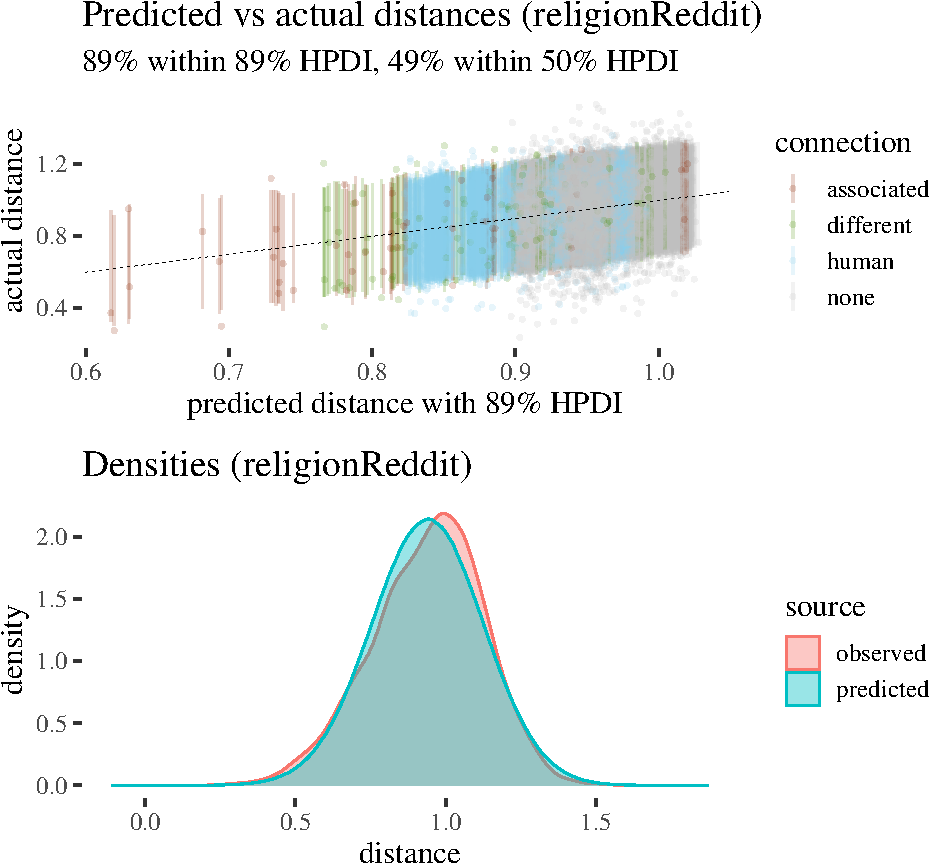
\includegraphics[width=0.8\linewidth]{paperDraft_files/figure-latex/figposteriorPrCheckA6b-1} \end{center}
\caption{Example of a posterior predictive check. (Left) Actual cosine distances are plotted against mean predictions with 89\% highest posterior density intervals. Notice that 90\% of actual values fall within the 89\% HPDI and 55\% of actual values fall into 50\% HPDI, which indicates appropriate performance of the model. The left-right alignment of differrent colors coressponds to the fact that cosine differences between elements of different categories differ, to some extent systematically (this will be studied in the results section). (Right) Densities of predicted and observed distances.}
\label{fig:posteriorCheck1}
\end{figure}

\normalsize

\hypertarget{results-and-discussion}{%
\section{Results and discussion}\label{results-and-discussion}}

\vspace{1mm}
\footnotesize

\hypertarget{observations}{%
\subsection{Observations}\label{observations}}

In brief, despite one-number metrics suggesting otherwise, our Bayesian
analysis reveals that insofar as the short word lists usually used in
related research projects are involved, there usually are no strong
reasons to claim the presence of systematic bias. Moreover, comparison
between the groups (including control word lists) leads to the
conclusion that the effect sizes (that is, the absolute differences
between cosine distances between groups) tend to be rather small, with
few exceptions. Moreover, the choice of protected words is crucial ---
as there is a lot of variance when it comes to the protected word-level
analysis.

In a bit more detail, the visualizations in Appendix
\ref{appendix:visualizations} show that the situation is more
complicated than merely looking at one-number summaries might suggest.
Note that the axes are sometimes in different scales to increase
visibility.

To start with, let us look at the association-type level coefficients
(illustrated in the top parts of the plots). Depending on the corpus
used and word class, there is a large variety as to the posterior
densities. Quite aware of this being a crude approximation, let's
compare the HPDIs and whether they overlap for different attribute
groups.

\begin{itemize}
\item
  In Weat 7 (Reddit) there is no reason to think there are systematic
  differences between cosine distances (recall that words from Weat 7
  were mostly not available in other embeddings).
\item
  In Weat 1 (Google, Glove and Reddit) associated words are somewhat
  closer, but the cosine distance differences from neutral words are
  very low, and surprisingly it is human attributes, not neutral
  predicates that are systematically the furthest.
\item
  In Religion (Google, Glove, Reddit) and Race (Google, Glove), the
  associated attributes are not systematically closer than attributes
  belonging to different stereotypes, and the difference from neutral
  and human predicates is rather low, if noticeable. The situation is
  interestingly different in Race (Reddit) where both human and neutral
  predicates are systematically further than associated and different
  attributes - but even then, there is no clear difference between
  associated and different attributes.
\item
  For Gender (Google, Glove), despite the superficially binary nature,
  associated and opposite attributes tend to be more or less in the same
  distances, much closer than neutral words (but not closer than human
  predicates in Glove). Reddit is an extreme example: both associated
  and opposite attributes are much closer than neutral and human (around
  .6 vs.~.9), but even then, there seems to be no reason to think than
  cosine distances to associated predicates are much different from
  distances to opposite predicates.
\end{itemize}

Moreover, when we look at particular protected words, the situation is
even less straightforward. We will just go over a few notable examples,
leaving the visual inspection of particular results for other protected
words to the reader. One general phenomenon is that--as we already
pointed out--the word lists are quite short, which contributes to large
uncertainty involved in some cases.

\begin{itemize}
\item
  For some protected words the different attributes are somewhat closer
  than the associated attributes.
\item
  For some protected words, associated and different attributes are
  closer than neutral attributes, but so are human attributes.
\item
  In some cases, associated attributes are closer, but so are neutral
  and human predicates, which illustrates that just looking at average
  cosine similarity as compared to the theoretically expected value of
  1, instead of running comparison to neutral and human attributes is
  misleading.
\item
  The only group of protected words where differences are noticeable at
  the protected word level is Gender-related words-- as in Gender
  (Google) and in Gender (Reddit) --- note however that in the latter,
  for some words the opposite attributes seem to be a little bit closer
  than the associated ones.
\end{itemize}

\hypertarget{rethinking-debiasing}{%
\subsection{Rethinking debiasing}\label{rethinking-debiasing}}

These visualizations can be also handy when it comes to the
investigation of the effect that debiasing has on the embedding space.
Below one may see chosen pair depicting the difference in means with
89\% highest posterior density intervals before and after applying
debiasing.

\begin{figure}[H]

\begin{center}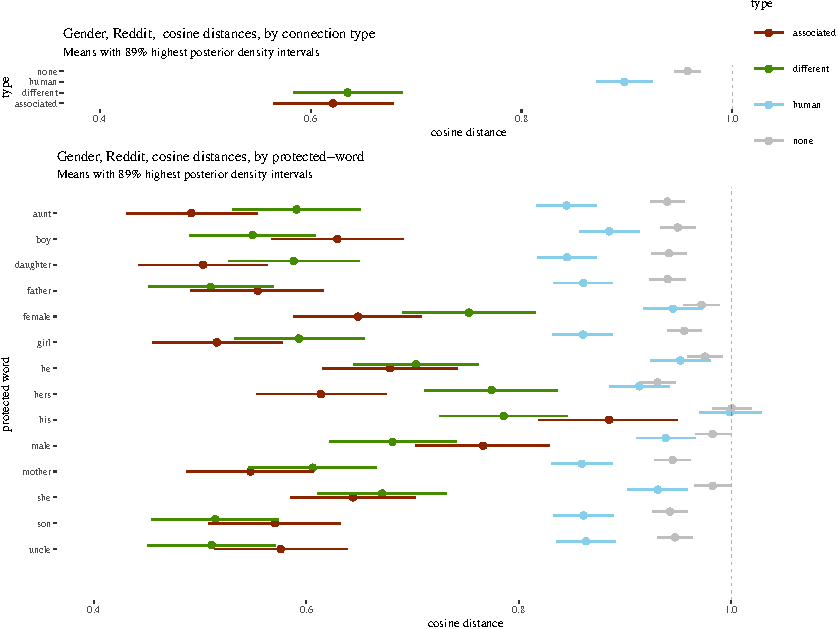
\includegraphics[width=0.85\linewidth]{paperDraft_files/figure-latex/fig:debiasedCosinePair2-1} 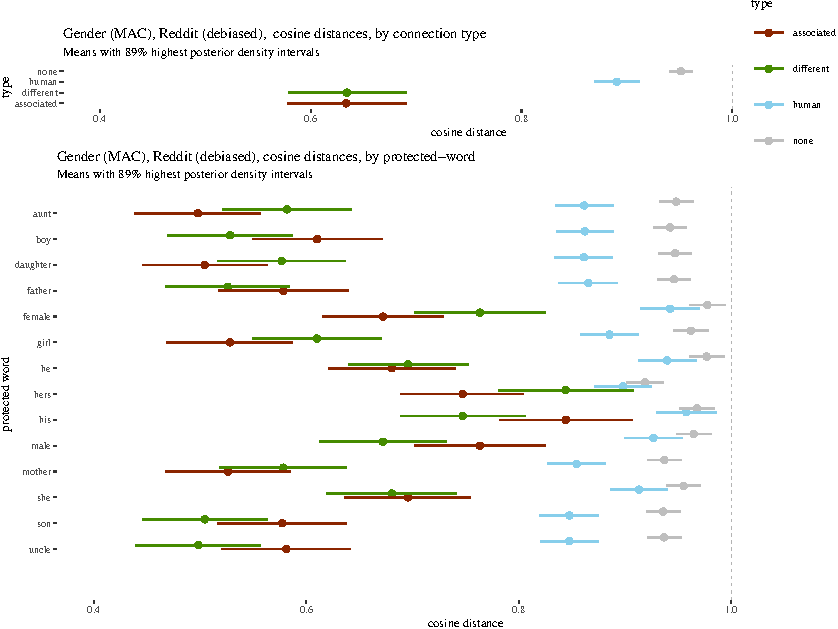
\includegraphics[width=0.85\linewidth]{paperDraft_files/figure-latex/fig:debiasedCosinePair2-2} \end{center}
\caption{Means with 89\% highest posterior density intervals for gender before and after debiasing.}
\label{fig:empiricalDebiasedPair}
\end{figure}

In Figure \ref{fig:empiricalDebiased} we look at the empirical
distributions for the debiased embeddings. Comparing the results to the
original embedding, one may notice that for the Religion group the
neutral and human distribution has changed slightly. Before within the
``correct'' cosine similarity boundaries there were 56\% of neutral and
55\% of human word lists. After the debiasing the values changed to 59\%
(for neutral) and 59\% (for human). The different and associated word
lists were more influenced. The general shape of both distributions is
less stretched. Before debiasing 43\% of the different word lists and
35\% of the associated word lists were within the accepted boundaries.
After the embedding manipulation the percentage has increased for both
lists to 63\%. Visualization for Gender group illustrates almost no
change for the neutral and human word lists before and after debiasing.
The values for different and associated word lists are also barely
impacted by the embedding modification. In the Race group, the
percentage within the boundaries for neutral and associated word lists
have increased. The opposite happened for human and different word
lists, where the percentage of ``correct'' cosine similarity dropped
from 67\% to 55\% (human) and from 39\% to 36\% (different).

\pagebreak

\begin{figure}[H]

\begin{center}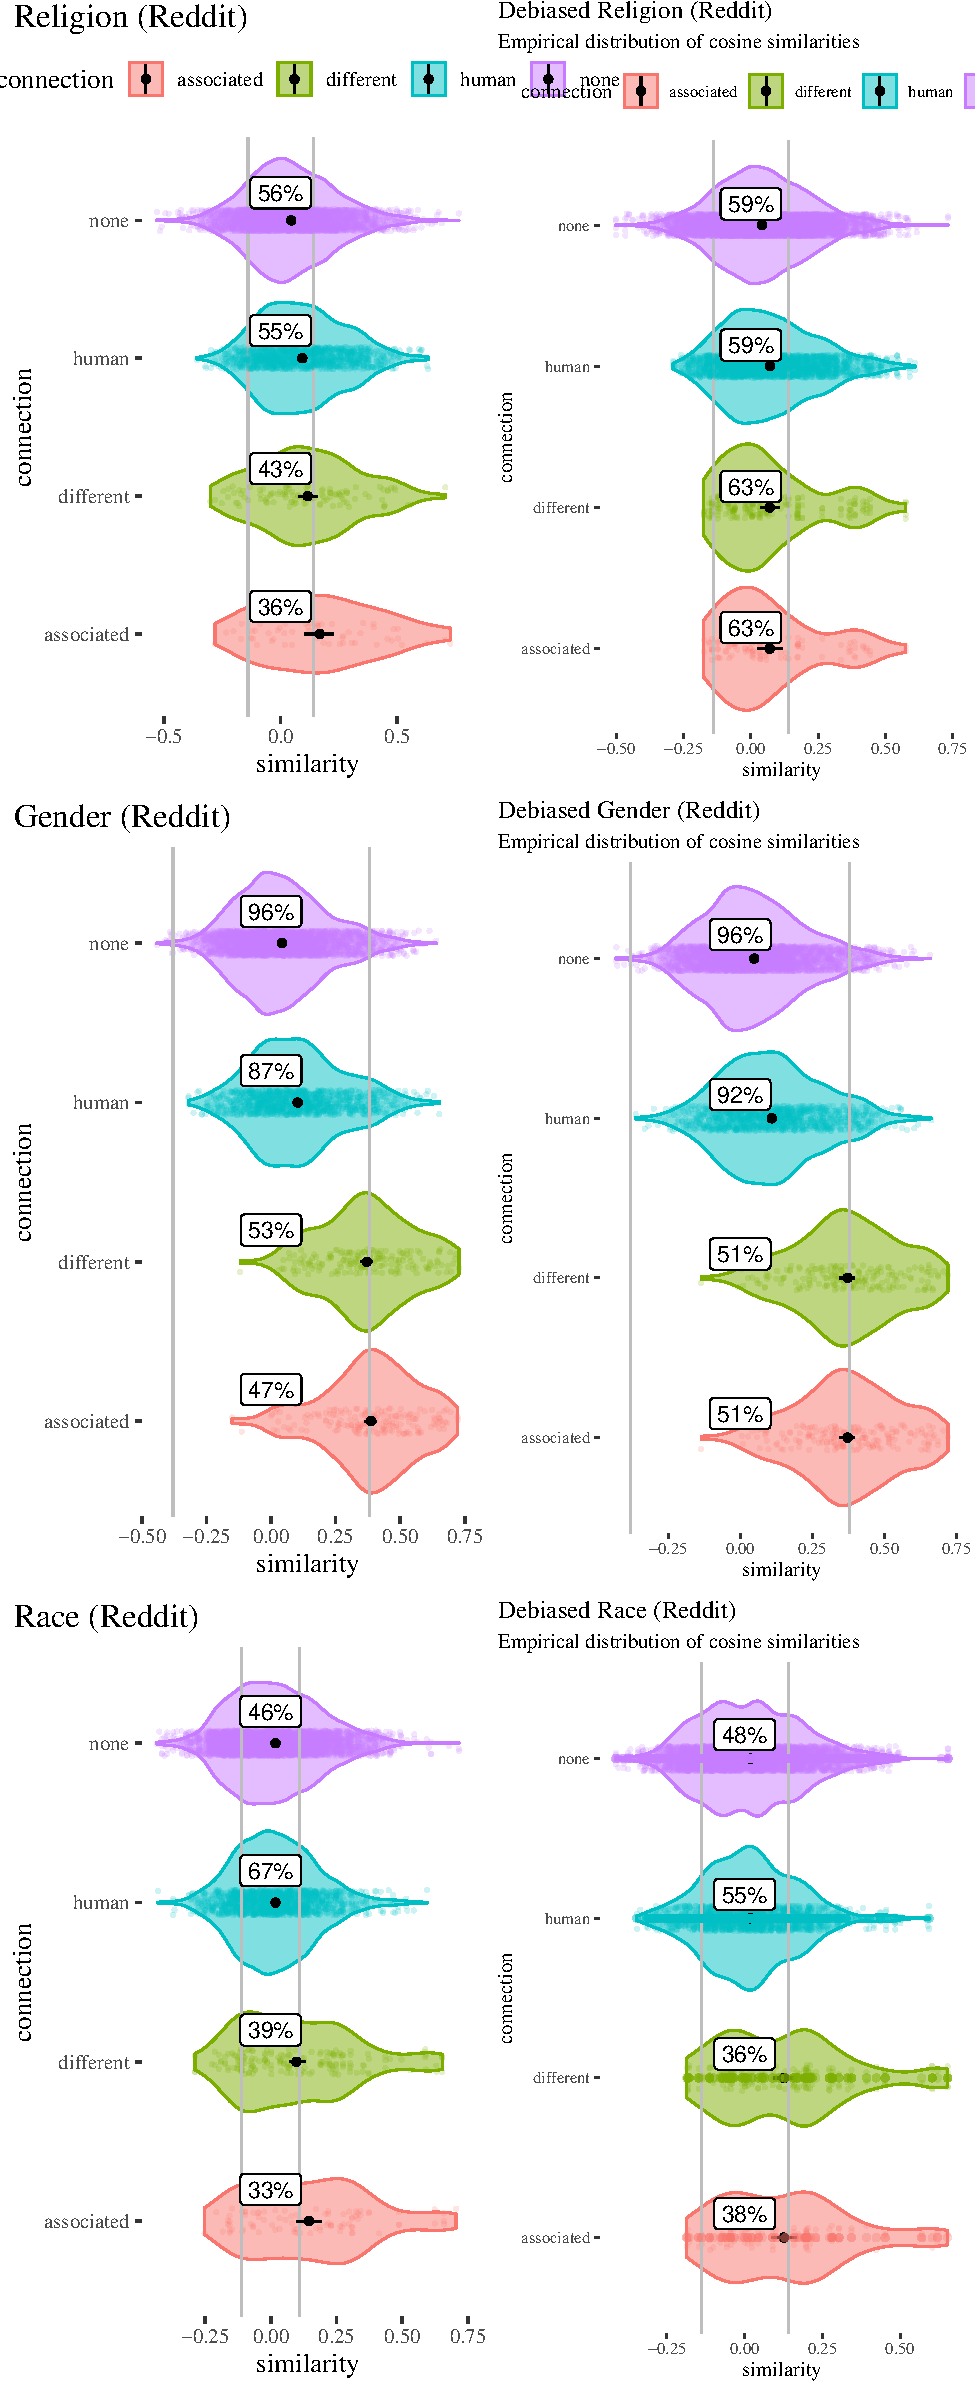
\includegraphics[width=0.7\linewidth]{paperDraft_files/figure-latex/fig:debiasedCosine-1} \end{center}
\caption{Empirical distributions of debiased cosine similarities (1-distances) for three word lists used in  the original paper.}
\label{fig:empiricalDebiased}
\end{figure}

\hypertarget{related-work-and-conclusions}{%
\section{Related work and
conclusions}\label{related-work-and-conclusions}}

It has been suggested {[}2{]} to use Bernstein bounds to state the
uncertainty of the sample bias in a form of confidence interval. The
interpretation of this interval is as follows, 95\% confidence interval
contains such a range of values, that one can be 95\% certain that it
contains the population mean. As we will prove later in the text,
confidence intervals are quite problematic for several reasons, among
others the confusing interpretability. In {[}2{]} the current problem of
bias estimation was correctly identified. Indeed, the bias estimate
should not be expressed as a single number without taking into account
that the estimate is made on a sample of data and therefore has
intrinsic uncertainty. However, we argue that Bernstein bounds do not
provide the best solution to this problem. Applying their method to a
popular WinoBias dataset leads to the conclusion that more than 11903
samples are needed to claim a 95\% confidence interval for a bias
estimate. This amount exceeds existing datasets for bias measurement. We
propose a more realistic method that can be applied to commonly used
datasets to estimate the uncertainty of the bias measurement.

\todo{More references to similar papers}

A Bayesian data analysis with hierarchical models of cosine distances
between protected words, control group words, and stereotypical
attributes provides more modest and realistic assessment of the
uncertainty involved. It reveals that much complexity is hidden when one
instead chases single bias metrics present in the literature.

After introducing the method, we apply it to multiple word embeddings
and results of supposed debiasing, putting forward some general
observations that are not exactly in line with the usual picture painted
in terms of WEAT or MAC (and the problem generalizes to any approach
that focuses on chasing a single numeric metric): the word list sizes
and sample sizes used in the studies are usually
small,\footnote{Depending on a list for [@Caliskan2017semanticsBiases] the range for protected words is between 13 and 100, and for attributes between 16 and 25; for [@Manzini2019blackToCriminal] the range for protected words is between 14 and 18, and for attributes between 11 and 25}
posterior density intervals are fairly wide, often the differences
between associated, different and neutral human predicates, are not very
impressive. Also, a preliminary inspection suggests that the
desirability of changes obtained by the usual debiasing methods is
debatable. The tools that we propose, however, allow for a more
fine-grained and multi-level evaluation of bias and debiasing in
language models without losing modesty about the uncertainties involved.

\newpage
\appendix

\hypertarget{appendix}{%
\section{Appendix}\label{appendix}}

\hypertarget{visualizations}{%
\subsection{Visualizations}\label{visualizations}}

\label{appendix:visualizations}

\begin{figure}[H]


\begin{center}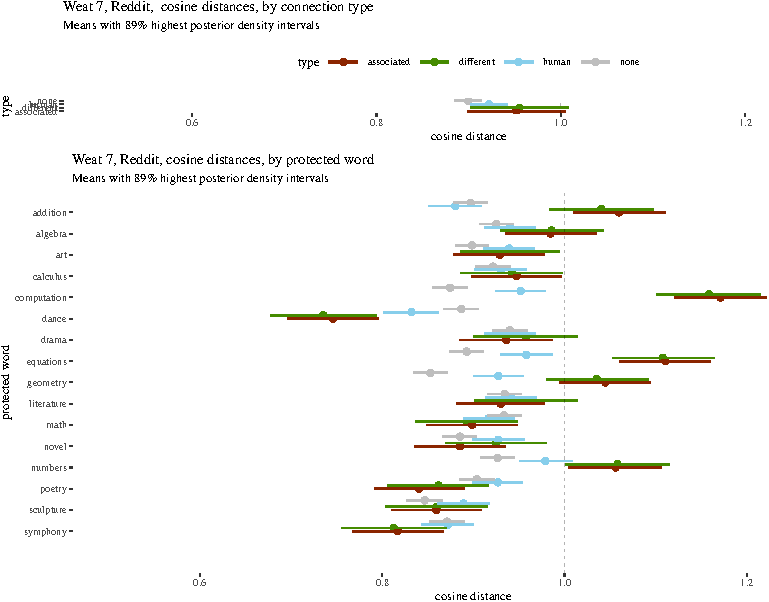
\includegraphics[width=1.1\linewidth]{paperDraft_files/figure-latex/unnamed-chunk-1-1} \end{center}
\caption{dsds}
\label{fig:weat7google}
\end{figure}

\begin{figure}[H]


\begin{center}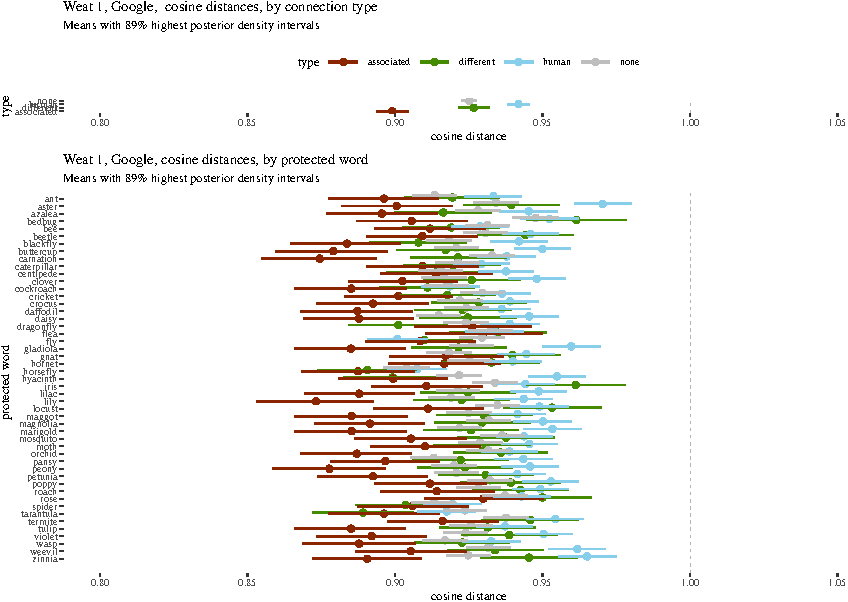
\includegraphics[width=1.1\linewidth]{paperDraft_files/figure-latex/unnamed-chunk-2-1} \end{center}
\caption{dsds}
\label{fig:weat7glove}
\end{figure}

\begin{figure}[H]


\begin{center}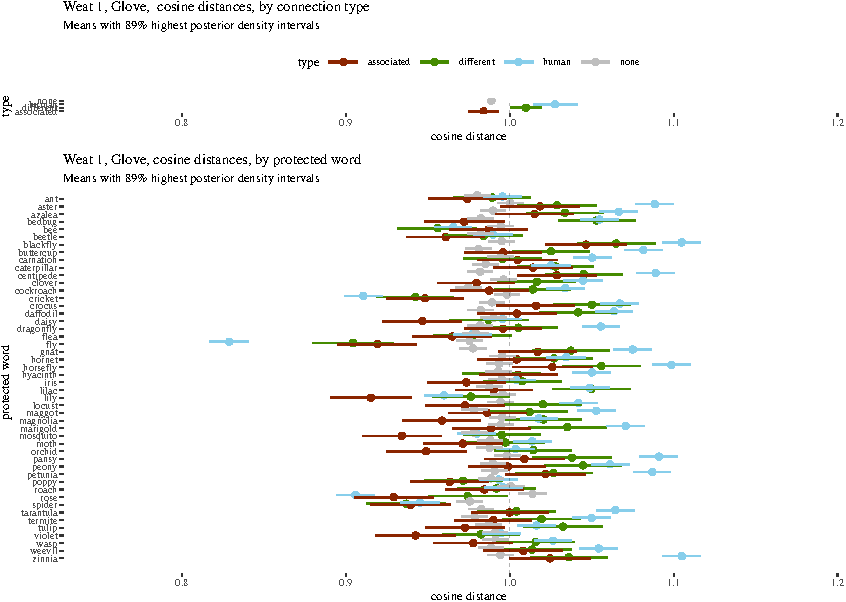
\includegraphics[width=1.1\linewidth]{paperDraft_files/figure-latex/unnamed-chunk-3-1} \end{center}
\caption{dsds}
\label{fig:weat7reddit}
\end{figure}

\begin{figure}[H]


\begin{center}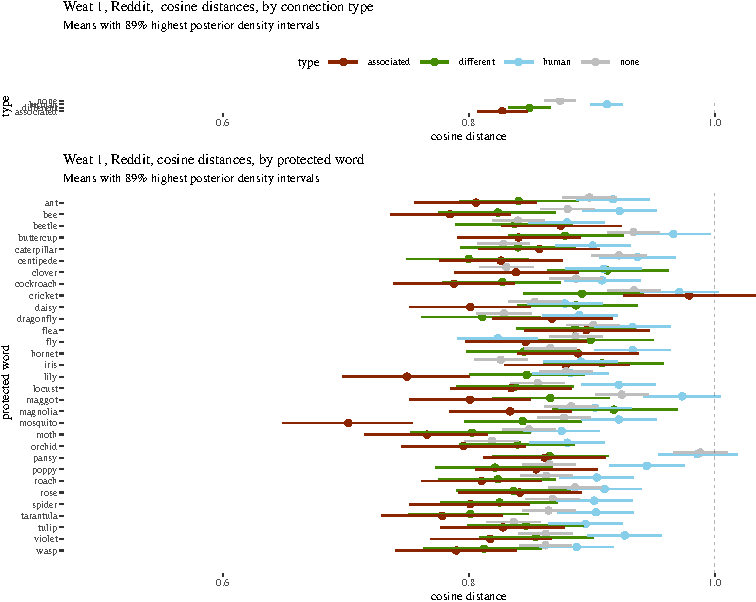
\includegraphics[width=1.1\linewidth]{paperDraft_files/figure-latex/unnamed-chunk-4-1} \end{center}
\caption{dsds}
\label{fig:weat1google}
\end{figure}

\begin{figure}[H]


\begin{center}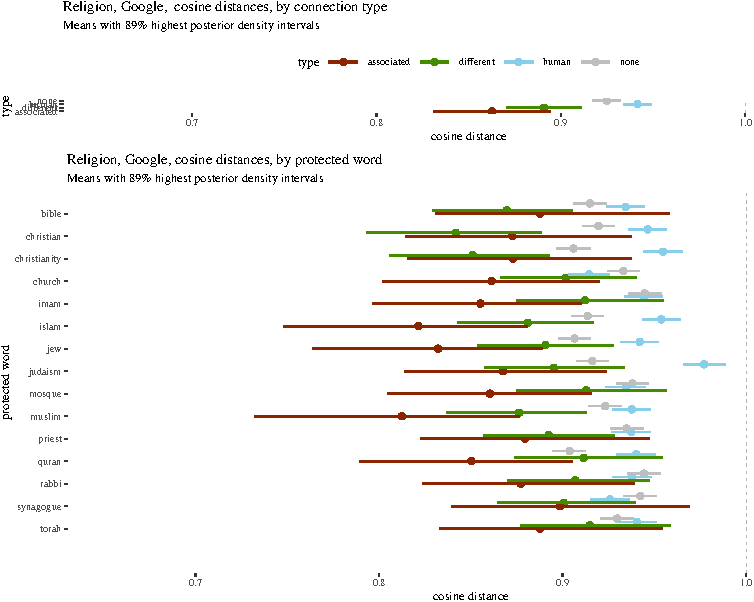
\includegraphics[width=1.1\linewidth]{paperDraft_files/figure-latex/unnamed-chunk-5-1} \end{center}
\caption{dsds}
\label{fig:weat1glove}
\end{figure}

\begin{figure}[H]


\begin{center}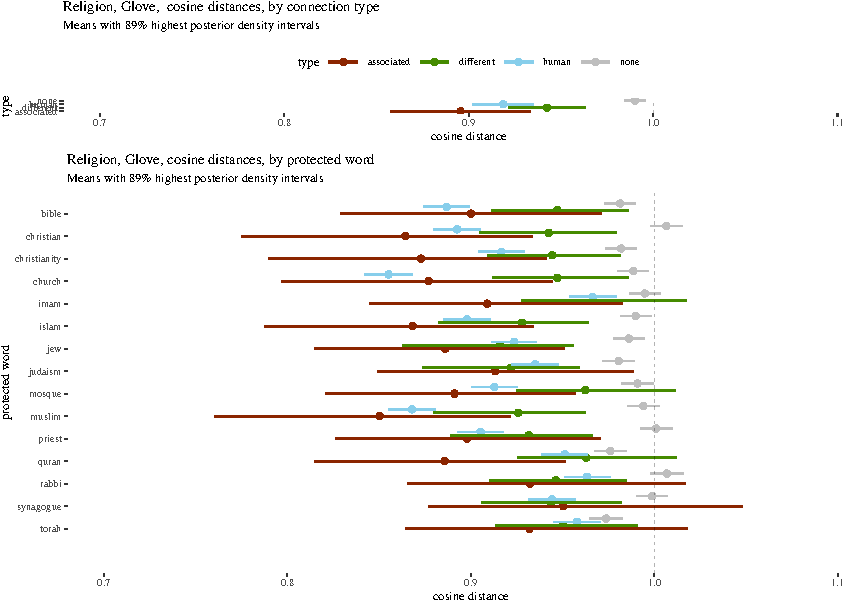
\includegraphics[width=1.1\linewidth]{paperDraft_files/figure-latex/unnamed-chunk-6-1} \end{center}
\caption{dsds}
\label{fig:weat1reddit}
\end{figure}

\begin{figure}[H]


\begin{center}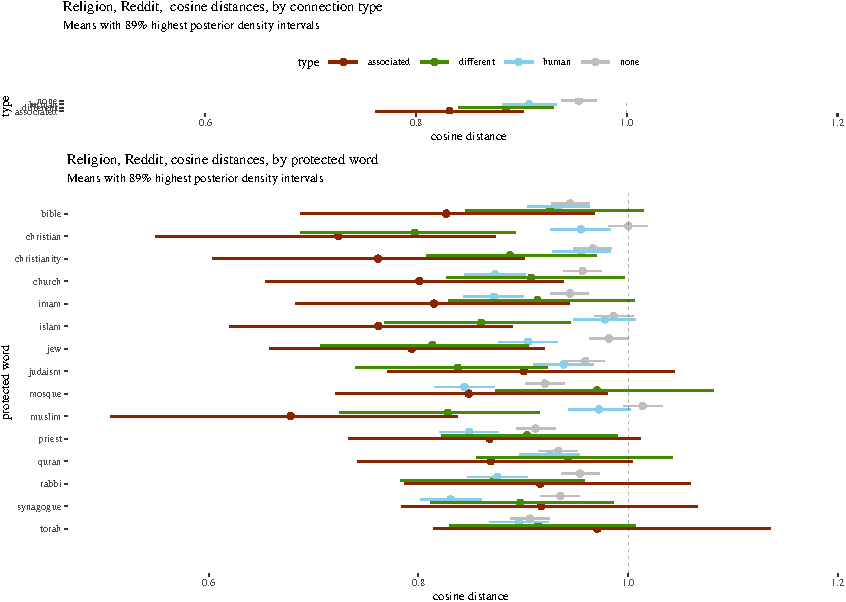
\includegraphics[width=1.1\linewidth]{paperDraft_files/figure-latex/unnamed-chunk-7-1} \end{center}
\caption{dsds}
\label{fig:religionGoogle}
\end{figure}

\begin{figure}[H]


\begin{center}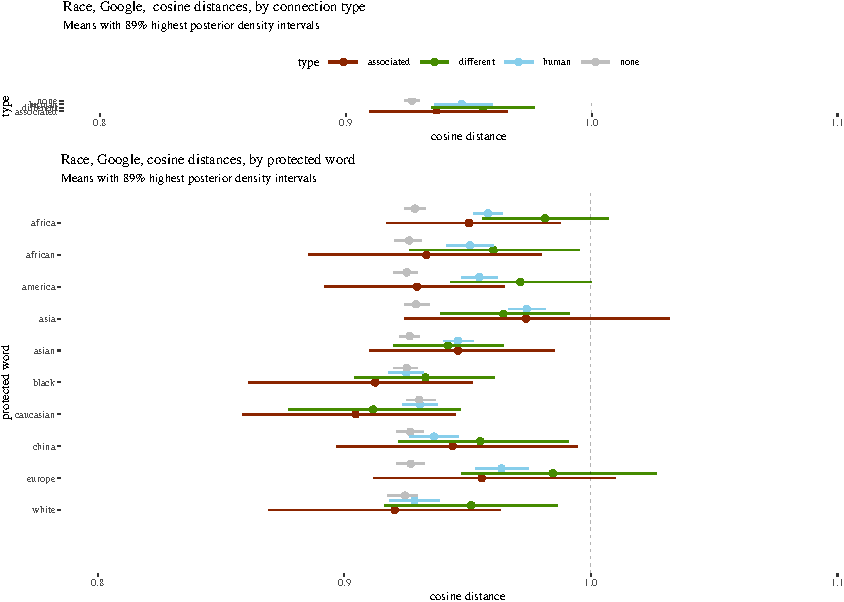
\includegraphics[width=1.1\linewidth]{paperDraft_files/figure-latex/unnamed-chunk-8-1} \end{center}
\caption{dsds}
\label{fig:religionGlove}
\end{figure}

\begin{figure}[H]


\begin{center}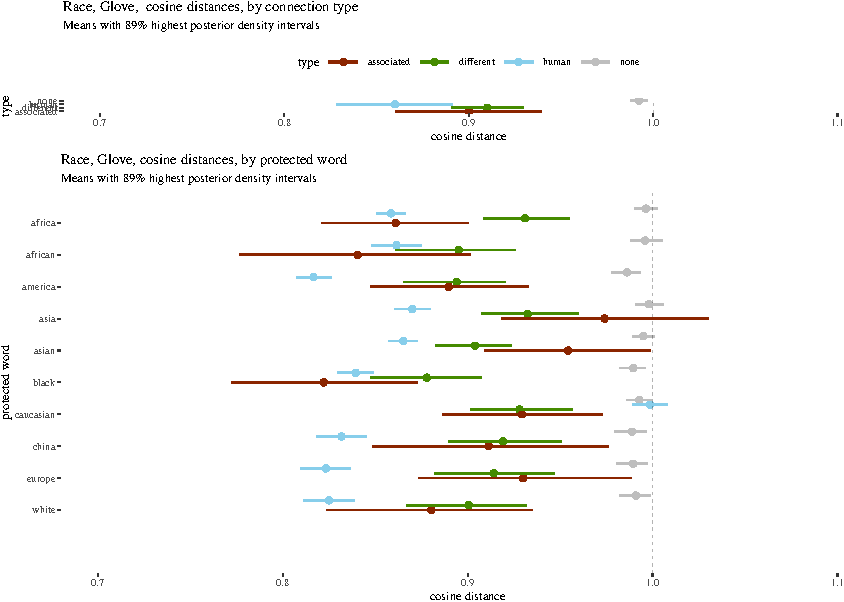
\includegraphics[width=1.1\linewidth]{paperDraft_files/figure-latex/unnamed-chunk-9-1} \end{center}
\caption{dsds}
\label{fig:religionReddit}
\end{figure}

\begin{figure}[H]


\begin{center}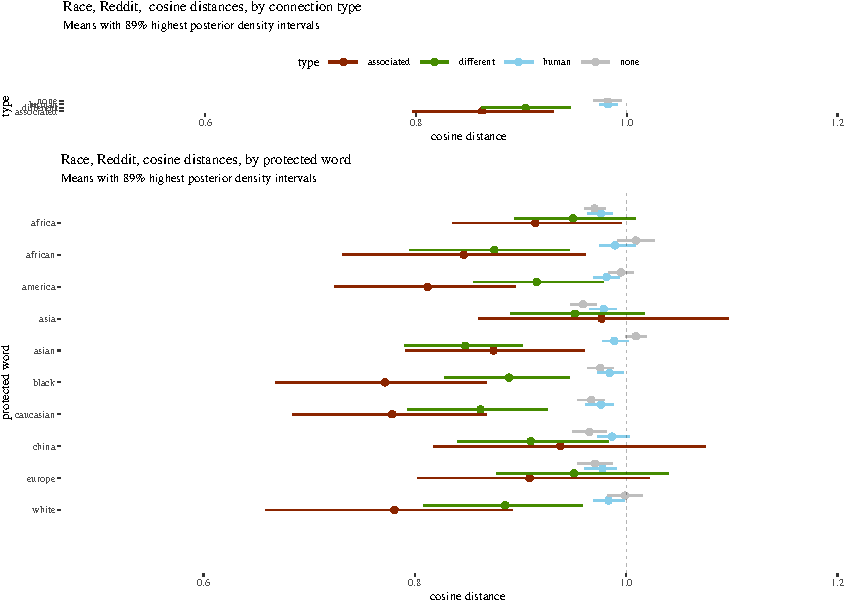
\includegraphics[width=1.1\linewidth]{paperDraft_files/figure-latex/unnamed-chunk-10-1} \end{center}
\caption{dsds}
\label{fig:raceGoogle}
\end{figure}

\begin{figure}[H]


\begin{center}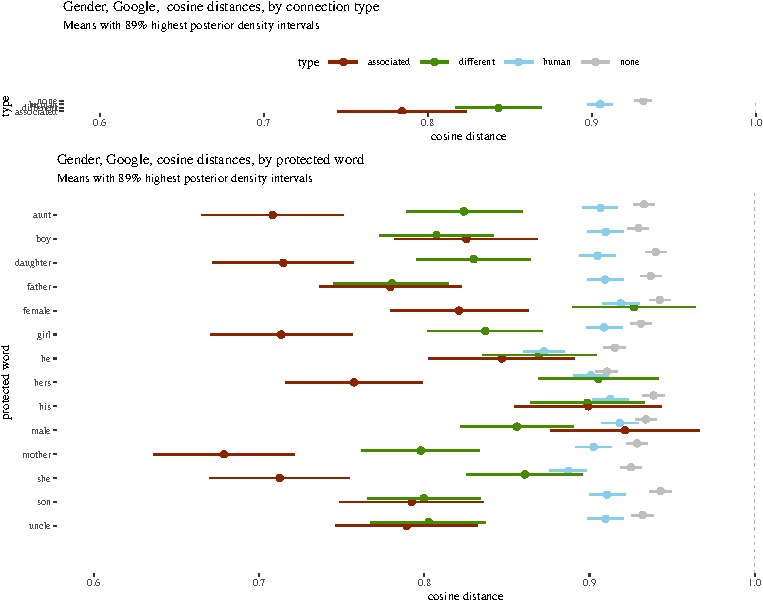
\includegraphics[width=1.1\linewidth]{paperDraft_files/figure-latex/unnamed-chunk-11-1} \end{center}
\caption{dsds}
\label{fig:raceGlove}
\end{figure}

\begin{figure}[H]


\begin{center}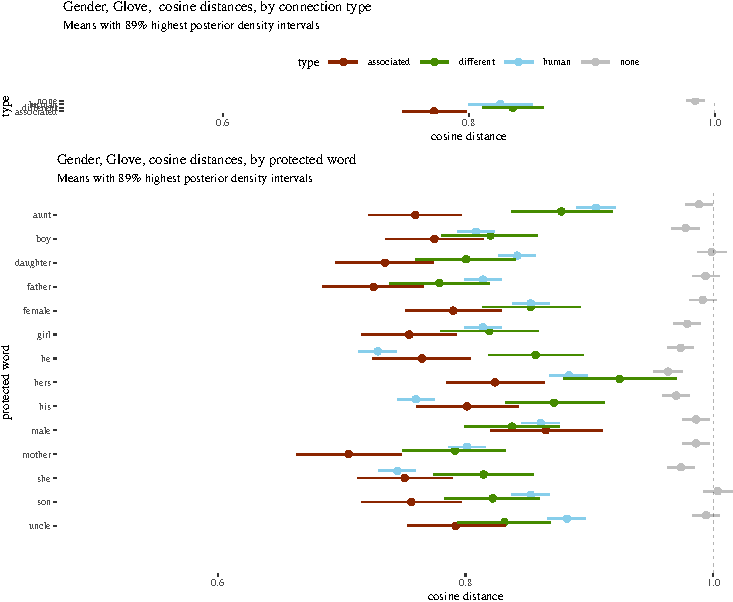
\includegraphics[width=1.1\linewidth]{paperDraft_files/figure-latex/unnamed-chunk-12-1} \end{center}
\caption{dsds}
\label{fig:raceReddit}
\end{figure}

\begin{figure}[H]


\begin{center}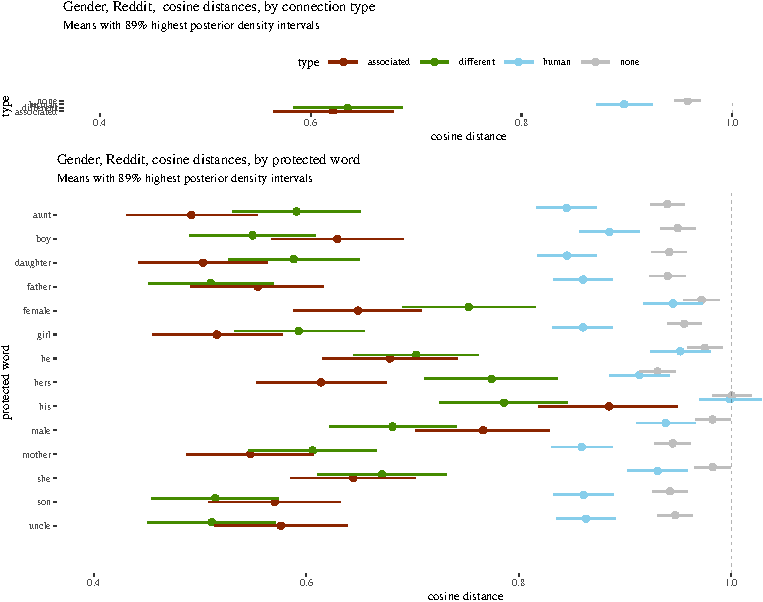
\includegraphics[width=1.1\linewidth]{paperDraft_files/figure-latex/unnamed-chunk-13-1} \end{center}
\caption{dsds}
\label{fig:genderGoogle}
\end{figure}

\begin{figure}[H]

\begin{center}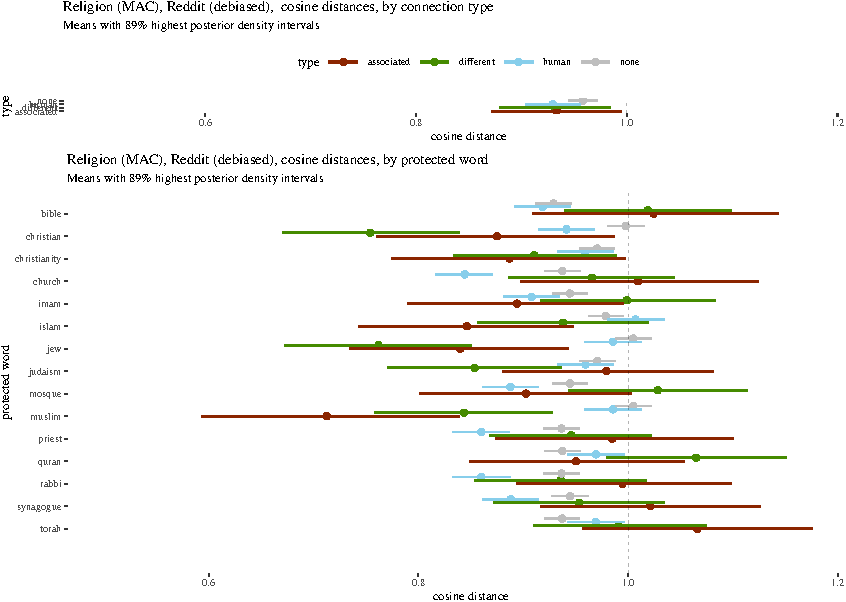
\includegraphics[width=1.1\linewidth]{paperDraft_files/figure-latex/unnamed-chunk-14-1} \end{center}
\caption{dsds}
\label{fig:genderGlove}
\end{figure}

\begin{figure}[H]

\begin{center}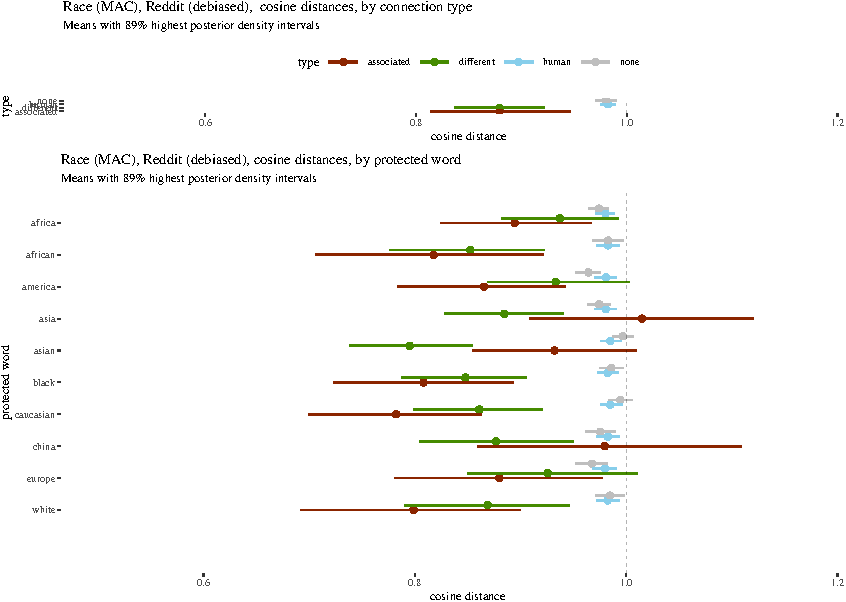
\includegraphics[width=1.1\linewidth]{paperDraft_files/figure-latex/unnamed-chunk-15-1} \end{center}
\caption{dsds}
\label{fig:genderReddit}
\end{figure}

\begin{figure}[H]

\begin{center}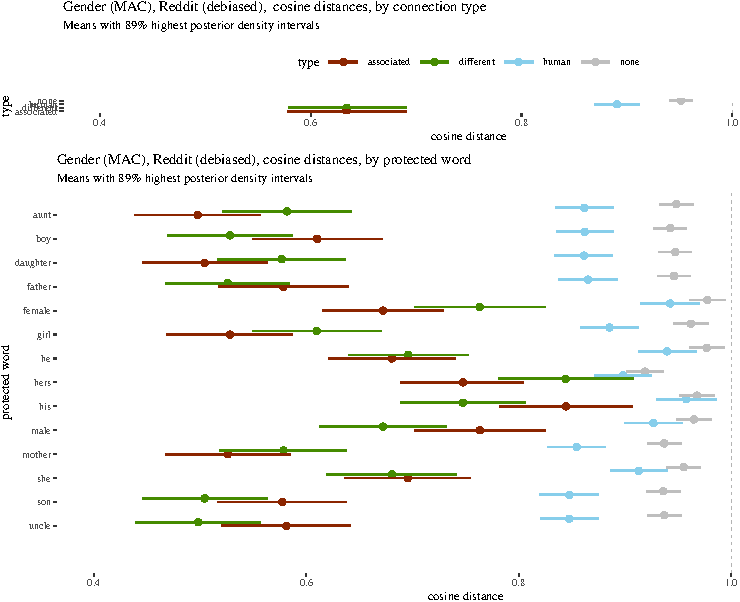
\includegraphics[width=1.1\linewidth]{paperDraft_files/figure-latex/unnamed-chunk-16-1} \end{center}
\caption{dsds}
\label{fig:debiasedReligion}
\end{figure}

\begin{figure}[H]

\begin{center}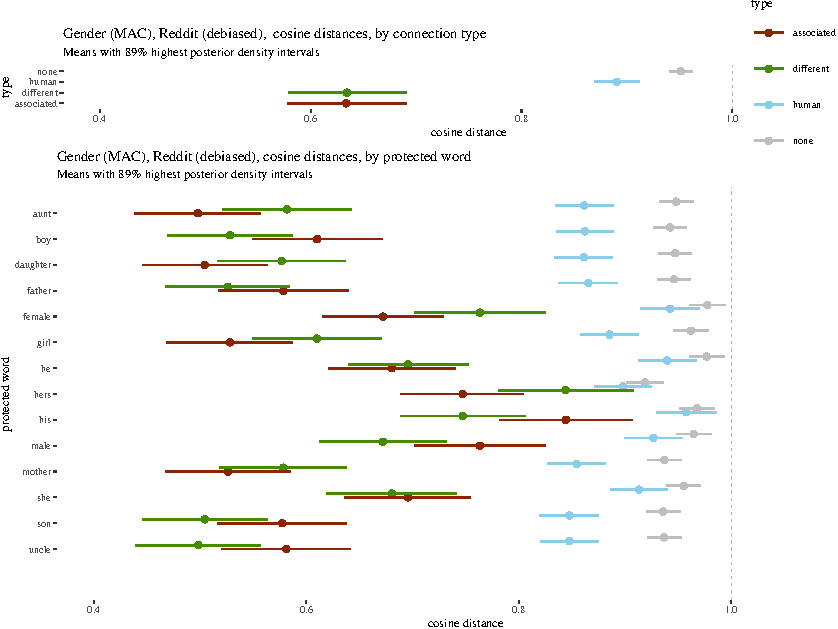
\includegraphics[width=1.1\linewidth]{paperDraft_files/figure-latex/unnamed-chunk-17-1} \end{center}
\caption{dsds}
\label{fig:debiasedRace}
\end{figure}

\begin{figure}[H]

\begin{center}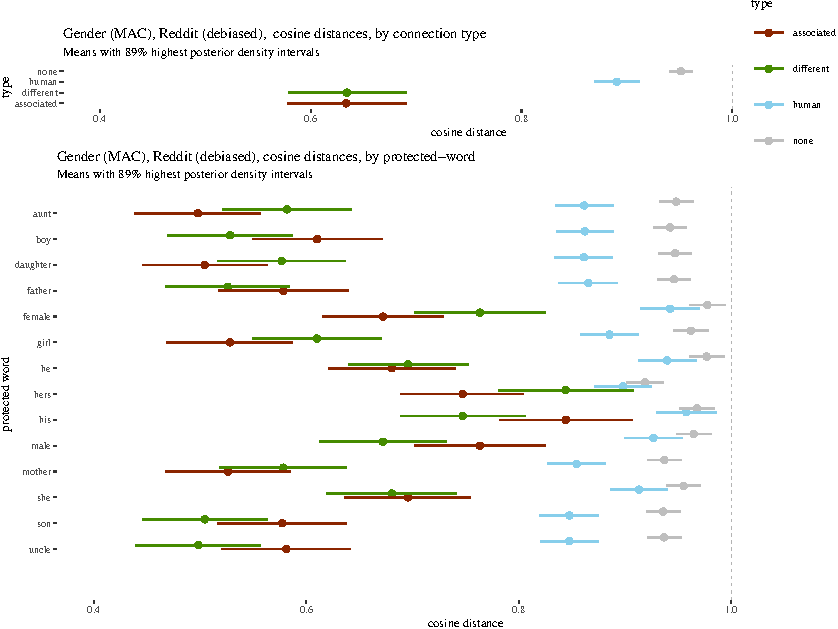
\includegraphics[width=1.1\linewidth]{paperDraft_files/figure-latex/unnamed-chunk-18-1} \end{center}
\caption{dsds}
\label{fig:debiasedGender}
\end{figure}

\hypertarget{posterior-predictive-checks}{%
\subsection{Posterior predictive
checks}\label{posterior-predictive-checks}}

\begin{center}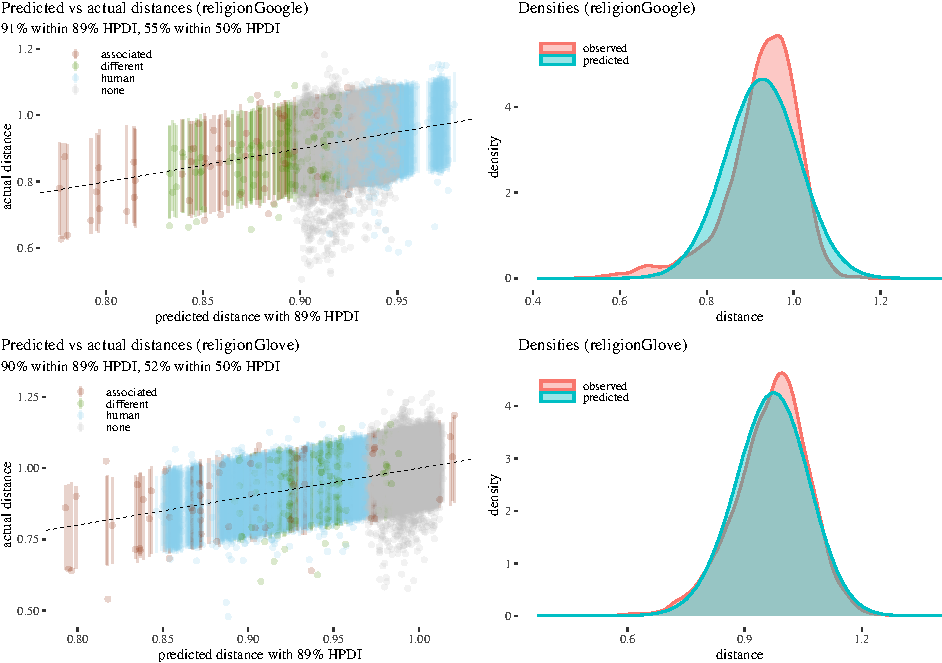
\includegraphics[width=0.85\linewidth,height=1\textheight]{paperDraft_files/figure-latex/figposteriorPrCheckAppendixa-1} \end{center}

\begin{center}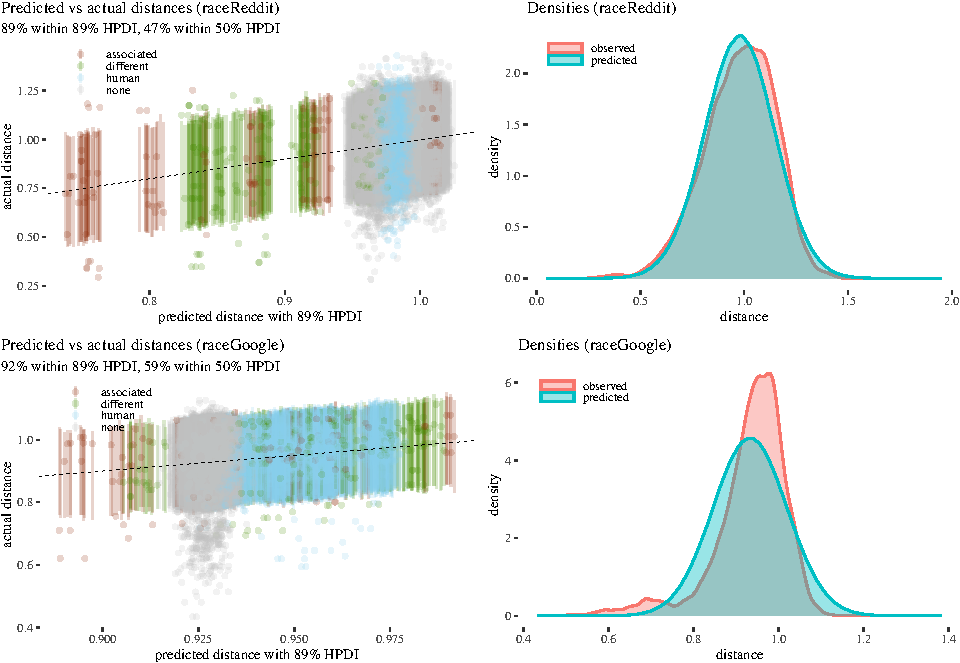
\includegraphics[width=0.85\linewidth,height=1\textheight]{paperDraft_files/figure-latex/figposteriorPrCheckAppendixb-1} \end{center}

\begin{center}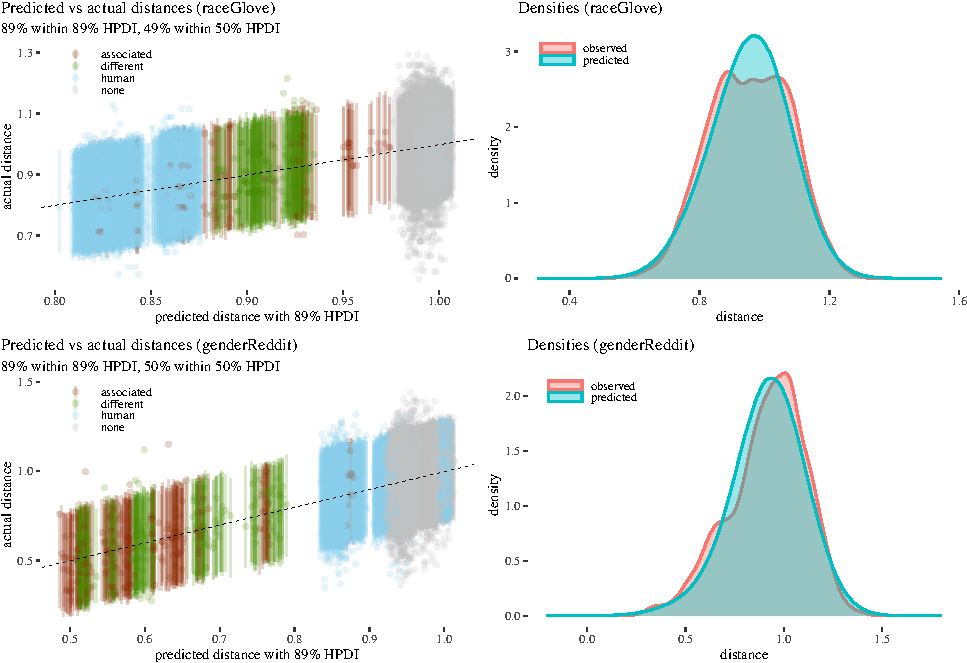
\includegraphics[width=0.87\linewidth,height=1\textheight]{paperDraft_files/figure-latex/figposteriorPrCheckAppendixc-1} \end{center}

\begin{center}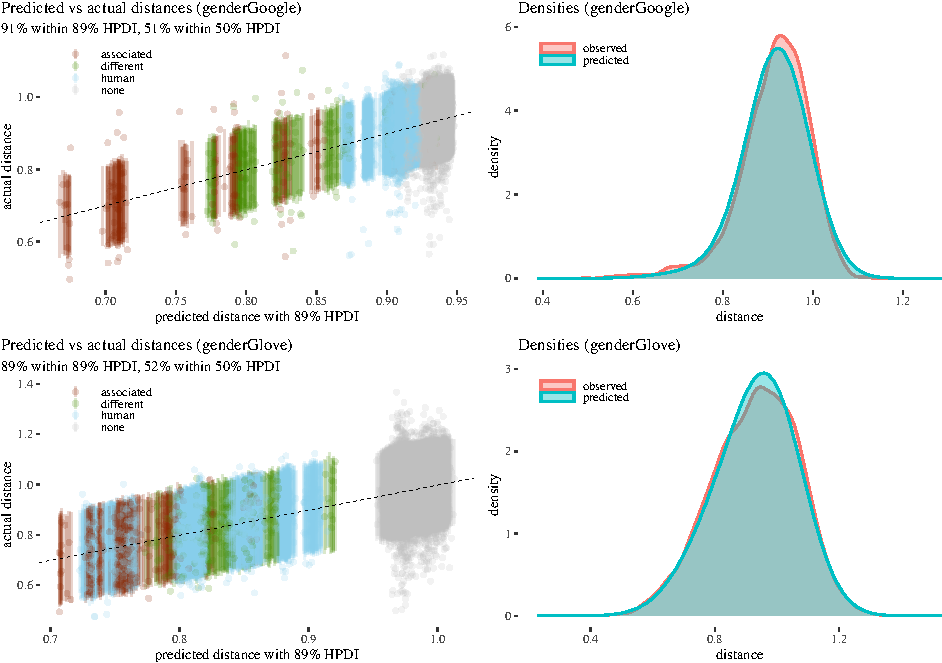
\includegraphics[width=0.89\linewidth,height=1\textheight]{paperDraft_files/figure-latex/figposteriorPrCheckAppendixd-1} \end{center}

\hypertarget{word-lists}{%
\subsection{Word lists}\label{word-lists}}

\hypertarget{lists-for-manzini2019blacktocriminal}{%
\subsubsection{Lists for
{[}12{]}:}\label{lists-for-manzini2019blacktocriminal}}

\label{appendix:manzini_word_lists} The lists are available here:

\begin{itemize}
\item
  \textbf{Gender:}
  \url{https://github.com/TManzini/DebiasMulticlassWordEmbedding/blob/master/Debiasing/data/vocab/gender_attributes_optm.json}
\item
  \textbf{Race:}
  \url{https://github.com/TManzini/DebiasMulticlassWordEmbedding/blob/master/Debiasing/data/vocab/race_attributes_optm.json}
\item
  \textbf{Religion:}
  \url{https://github.com/TManzini/DebiasMulticlassWordEmbedding/blob/master/Debiasing/data/vocab/religion_attributes_optm.json}
\end{itemize}

The lists are:

\begin{itemize}
\tightlist
\item
  \textbf{Gender:}
\end{itemize}

Pairs of protected attributes: {[}``he'', ``she''{]}, {[}``his'',
``hers''{]}, {[}``son'', ``daughter''{]}, {[}``father'', ``mother''{]},
{[}``male'', ``female''{]}, {[}``boy'', ``girl''{]}, {[}``uncle'',
``aunt''{]}

Lists of stereotypes per gender: man: {[}``manager'', ``executive'',
``doctor'', ``lawyer'', ``programmer'', ``scientist'', ``soldier'',
``supervisor'', ``rancher'', ``janitor'', ``firefighter'',
``officer''{]}, woman: {[}``secretary'', ``nurse'', ``clerk'',
``artist'', ``homemaker'', ``dancer'', ``singer'', ``librarian'',
``maid'', ``hairdresser'', ``stylist'', ``receptionist'',
``counselor''{]} \}

\begin{itemize}
\tightlist
\item
  \textbf{Race:}
\end{itemize}

Sets of protected attributes: {[}``black'', ``caucasian'', ``asian''{]},
{[}``african'', ``caucasian'', ``asian''{]}, {[}``black'', ``white'',
``asian''{]}, {[}``africa'', ``america'', ``asia''{]}, {[}``africa'',
``america'', ``china''{]}, {[}``africa'', ``europe'', ``asia''{]}

Lists of stereotypes per race: ``caucasian'': {[}``manager'',
``executive'', ``redneck'', ``hillbilly'', ``leader'', ``farmer''{]},
``asian'' : {[}``doctor'', ``engineer'', ``laborer'', ``teacher''{]},
``black'' : {[}``slave'', ``musician'', ``runner'', ``criminal'',
``homeless''{]}

\begin{itemize}
\tightlist
\item
  \textbf{Religion:}
\end{itemize}

Sets of protected attributes: {[}``judaism'', ``christianity'',
``islam''{]}, {[}``jew'', ``christian'', ``muslim''{]},
{[}``synagogue'', ``church'', ``mosque''{]}, {[}``torah'', ``bible'',
``quran''{]}, {[}``rabbi'', ``priest'', ``imam''{]}

Lists of stereotypes per race: ``jew'' : {[}``greedy'', ``cheap'',
``hairy'', ``liberal''{]}, ``christian'' : {[}``judgemental'',
``conservative'', ``familial''{]}, ``muslim'' : {[}``violent'',
``terrorist'', ``dirty'', ``uneducated''{]}

\hypertarget{our-custom-word-lists}{%
\subsubsection{Our custom word lists}\label{our-custom-word-lists}}

\begin{itemize}
\tightlist
\item
  \textbf{Neutral:}
\end{itemize}

{[}`ballpark', `glitchy', `billy', `dallas', `rip', `called',
`outlooks', `floater', `rattlesnake', `exports', `recursion',
`shortfall', `corrected', `solutions', `diagnostic', `patently',
`flops', `approx', `percents', `lox', `hamburger', `engulfed',
`households', `north', `playtest', `replayability', `glottal',
`parable', `gingers', `anachronism', `organizing', `reach', `shtick',
`eleventh', `cpu', `ranked', `irreversibly', `ponce', `velociraptor',
`defects', `puzzle', `smasher', `northside', `heft', `observation',
`rectum', `mystical', `telltale', `remnants', `inquiry', `indisputable',
`boatload', `lessening', `uselessness', `observes', `fictitious',
`repatriation', `duh', `attic', `schilling', `charges', `chatter',
`pad', `smurfing', `worthiness', `definitive', `neat', `homogenized',
`lexicon', `nationalized', `earpiece', `specializations', `lapse',
`concludes', `weaving', `apprentices', `fri', `militias',
`inscriptions', `gouda', `lift', `laboring', `adaptive', `lecture',
`hogging', `thorne', `fud', `skews', `epistles', `tagging', `crud',
`two', `rebalanced', `payroll', `damned', `approve', `reason',
`formally', `releasing', `muddled', `mineral', `shied', `capital',
`nodded', `escrow', `disconnecting', `marshals', `winamp', `forceful',
`lowes', `sip', `pencils', `stomachs', `goff', `cg', `backyard',
`uprooting', `merging', `helpful', `eid', `trenchcoat', `airlift',
`frothing', `pulls', `volta', `guinness', `viewership', `eruption',
`peeves', `goat', `goofy', `disbanding', `relented', `ratings',
`disputed', `vitamins', `singled', `hydroxide', `telegraphed',
`mercantile', `headache', `muppets', `petal', `arrange', `donovan',
`scrutinized', `spoil', `examiner', `ironed', `maia', `condensation',
`receipt', `solider', `tattooing', `encoded', `compartmentalize',
`lain', `gov', `printers', `hiked', `resentment', `revisionism',
`tavern', `backpacking', `pestering', `acknowledges', `testimonies',
`parlance', `hallucinate', `speeches', `engaging', `solder',
`perceptive', `microbiology', `reconnaissance', `garlic', `neutrals',
`width', `literaly', `guild', `despicable', `dion', `option',
`transistors', `chiropractic', `tattered', `consolidating', `olds',
`garmin', `shift', `granted', `intramural', `allie', `cylinders',
`wishlist', `crank', `wrongly', `workshop', `yesterday', `wooden',
`without', `wheel', `weather', `watch', `version', `usually', `twice',
`tomato', `ticket', `text', `switch', `studio', `stick', `soup',
`sometimes', `signal', `prior', `plant', `photo', `path', `park',
`near', `menu', `latter', `grass', `clock'{]}

\begin{itemize}
\tightlist
\item
  \textbf{Human-related:}
\end{itemize}

{[}`wear', `walk', `visitor', `toy', `tissue', `throw', `talk', `sleep',
`eye', `enjoy', `blogger', `character', `candidate', `breakfast',
`supper', `dinner', `eat', `drink', ``carry'', ``run'', ``cast'',
``ask'', ``awake'', ``ear'', ``nose'', ``lunch'', ``coalition'',
``policies'', ``restaurant'', ``stood'', ``assumed'', ``attend'',
``swimming'', ``trip'', ``door'', ``determine'', ``gets'', ``leg'',
``arrival'', ``translated'', ``eyes'', ``step'', ``whilst'',
``translation'', ``practices'', ``measure'', ``storage'', ``window'',
``journey'', ``interested'', ``tries'', ``suggests'', ``allied'',
``cinema'', ``finding'', ``restoration'', ``expression'',``visitors'',
``tell'', ``visiting'', ``appointment'', ``adults'', ``bringing'',
``camera'', ``deaths'', ``filmed'', ``annually'', ``plane'', ``speak'',
``meetings'', ``arm'', ``speaking'', ``touring'', ``weekend'',
``accept'', ``describe'', ``everyone'', ``ready'', ``recovered'',
``birthday'', ``seeing'', ``steps'', ``indicate'', ``anyone'',
``youtube''{]}

\hypertarget{refs}{}
\begin{CSLReferences}{0}{0}
\leavevmode\vadjust pre{\hypertarget{ref-Bolukbasi2016man}{}}%
\CSLLeftMargin{{[}1{]} }%
\CSLRightInline{Tolga Bolukbasi, Kai-Wei Chang, James Y. Zou, Venkatesh
Saligrama, and Adam Kalai. 2016. Man is to computer programmer as woman
is to homemaker? Debiasing word embeddings. \emph{CoRR} abs/1607.06520,
(2016). Retrieved from \url{http://arxiv.org/abs/1607.06520}}

\leavevmode\vadjust pre{\hypertarget{ref-Ethayarajh2020Bernstein}{}}%
\CSLLeftMargin{{[}2{]} }%
\CSLRightInline{Kawin Ethayarajh. 2020. Is your classifier actually
biased? Measuring fairness under uncertainty with bernstein bounds.
\emph{CoRR} abs/2004.12332, (2020). Retrieved from
\url{https://arxiv.org/abs/2004.12332}}

\leavevmode\vadjust pre{\hypertarget{ref-Garg2017hundredYears}{}}%
\CSLLeftMargin{{[}3{]} }%
\CSLRightInline{Nikhil Garg, Londa Schiebinger, Dan Jurafsky, and James
Zou. 2017. Word embeddings quantify 100 years of gender and ethnic
stereotypes. \emph{Proceedings of the National Academy of Sciences} 115,
(November 2017).
DOI:https://doi.org/\href{https://doi.org/10.1073/pnas.1720347115}{10.1073/pnas.1720347115}}

\leavevmode\vadjust pre{\hypertarget{ref-Garg2018years}{}}%
\CSLLeftMargin{{[}4{]} }%
\CSLRightInline{Nikhil Garg, Londa Schiebinger, Dan Jurafsky, and James
Zou. 2018. Word embeddings quantify 100 years of gender and ethnic
stereotypes. \emph{Proceedings of the National Academy of Sciences} 115,
16 (April 2018), E3635--E3644.
DOI:https://doi.org/\href{https://doi.org/10.1073/pnas.1720347115}{10.1073/pnas.1720347115}}

\leavevmode\vadjust pre{\hypertarget{ref-Gonen2019lipstick}{}}%
\CSLLeftMargin{{[}5{]} }%
\CSLRightInline{Hila Gonen and Yoav Goldberg. 2019. Lipstick on a pig:
{D}ebiasing methods cover up systematic gender biases in word embeddings
but do not remove them. In \emph{Proceedings of the 2019 conference of
the north {A}merican chapter of the association for computational
linguistics: Human language technologies, volume 1 (long and short
papers)}, Association for Computational Linguistics, Minneapolis,
Minnesota, 609--614.
DOI:https://doi.org/\href{https://doi.org/10.18653/v1/N19-1061}{10.18653/v1/N19-1061}}

\leavevmode\vadjust pre{\hypertarget{ref-gordon2012reporting}{}}%
\CSLLeftMargin{{[}6{]} }%
\CSLRightInline{Jonathan Gordon and Benjamin Durme. 2013. Reporting bias
and knowledge acquisition. In \emph{AKBC 2013 - Proceedings of the 2013
Workshop on Automated Knowledge Base Construction, Co-located with CIKM
2013}, 25--30.
DOI:https://doi.org/\href{https://doi.org/10.1145/2509558.2509563}{10.1145/2509558.2509563}}

\leavevmode\vadjust pre{\hypertarget{ref-Hoekstra2014Misinterpretation}{}}%
\CSLLeftMargin{{[}7{]} }%
\CSLRightInline{Rink Hoekstra, Richard D. Morey, Jeffrey N. Rouder, and
Eric-Jan Wagenmakers. 2014. Robust misinterpretation of confidence
intervals. \emph{Psychonomic Bulletin \& Review} 21, 5 (October 2014),
1157--1164.
DOI:https://doi.org/\href{https://doi.org/10.3758/s13423-013-0572-3}{10.3758/s13423-013-0572-3}}

\leavevmode\vadjust pre{\hypertarget{ref-Caliskan2017semanticsBiases}{}}%
\CSLLeftMargin{{[}8{]} }%
\CSLRightInline{Aylin Caliskan Islam, Joanna J. Bryson, and Arvind
Narayanan. 2016. Semantics derived automatically from language corpora
necessarily contain human biases. \emph{CoRR} abs/1608.07187, (2016).
Retrieved from \url{http://arxiv.org/abs/1608.07187}}

\leavevmode\vadjust pre{\hypertarget{ref-JohnsonValueFree}{}}%
\CSLLeftMargin{{[}9{]} }%
\CSLRightInline{Gabbrielle Johnson. forthcoming. Are algorithms
value-free? Feminist theoretical virtues in machine learning.
\emph{Journal Moral Philosophy} (forthcoming).}

\leavevmode\vadjust pre{\hypertarget{ref-kruschke2015bayesian}{}}%
\CSLLeftMargin{{[}10{]} }%
\CSLRightInline{John Kruschke. 2015. \emph{Doing bayesian data analysis
(second edition)}. Academic Press, Boston.}

\leavevmode\vadjust pre{\hypertarget{ref-Lauscher2019multidimensional}{}}%
\CSLLeftMargin{{[}11{]} }%
\CSLRightInline{Anne Lauscher and Goran Glavas. 2019. Are we
consistently biased? Multidimensional analysis of biases in
distributional word vectors. \emph{CoRR} abs/1904.11783, (2019).
Retrieved from \url{http://arxiv.org/abs/1904.11783}}

\leavevmode\vadjust pre{\hypertarget{ref-Manzini2019blackToCriminal}{}}%
\CSLLeftMargin{{[}12{]} }%
\CSLRightInline{Thomas Manzini, Yao Chong Lim, Yulia Tsvetkov, and Alan
W Black. 2019. Black is to criminal as caucasian is to police: Detecting
and removing multiclass bias in word embeddings. Retrieved from
\url{https://arxiv.org/abs/1904.04047}}

\leavevmode\vadjust pre{\hypertarget{ref-statrethinkingbook2020}{}}%
\CSLLeftMargin{{[}13{]} }%
\CSLRightInline{Richard McElreath. 2020. \emph{Statistical rethinking: A
bayesian course with examples in r and stan, 2nd edition} (2nd ed.). CRC
Press. Retrieved from
\url{http://xcelab.net/rm/statistical-rethinking/}}

\leavevmode\vadjust pre{\hypertarget{ref-Mikolov2013efficient}{}}%
\CSLLeftMargin{{[}14{]} }%
\CSLRightInline{Tomas Mikolov, Kai Chen, Greg Corrado, and Jeffrey Dean.
2013. Efficient estimation of word representations in vector space.
DOI:https://doi.org/\href{https://doi.org/10.48550/ARXIV.1301.3781}{10.48550/ARXIV.1301.3781}}

\leavevmode\vadjust pre{\hypertarget{ref-Morey2015confidenceFallacy}{}}%
\CSLLeftMargin{{[}15{]} }%
\CSLRightInline{Richard Morey, Rink Hoekstra, Jeffrey Rouder, Michael
Lee, and EJ Wagenmakers. 2015. The fallacy of placing confidence in
confidence intervals. \emph{Psychonomic Bulletin \& Review} (September
2015).}

\leavevmode\vadjust pre{\hypertarget{ref-Nissim2020fair}{}}%
\CSLLeftMargin{{[}16{]} }%
\CSLRightInline{Malvina Nissim, Rik van Noord, and Rob van der Goot.
2020. Fair is better than sensational: Man is to doctor as woman is to
doctor. \emph{Computational Linguistics} 46, 2 (June 2020), 487--497.
DOI:https://doi.org/\href{https://doi.org/10.1162/coli_a_00379}{10.1162/coli\_a\_00379}}

\leavevmode\vadjust pre{\hypertarget{ref-Nosek2002harvesting}{}}%
\CSLLeftMargin{{[}17{]} }%
\CSLRightInline{Brian A. Nosek, Mahzarin R. Banaji, and Anthony G.
Greenwald. 2002. Harvesting implicit group attitudes and beliefs from a
demonstration web site. \emph{Group Dynamics: Theory, Research, and
Practice} 6, 1 (2002), 101--115.
DOI:https://doi.org/\href{https://doi.org/10.1037/1089-2699.6.1.101}{10.1037/1089-2699.6.1.101}}

\end{CSLReferences}

\end{document}
